%%%%%%%%%%%%%%%%%%%%%%%%%%%%%% -*- Mode: Latex -*- %%%%%%%%%%%%%%%%%%%%%%%%%%%%
%% 06-12.tex -- Thesis Pre-Proposal for Ph.D
%% Author          : Hongbing Kou
%% Created On      : Mon Sep 23 11:52:28 2002
%% Last Modified By: Hongbing Kou
%% Last Modified On: Fri Mar 16 15:47:24 2007
%% RCS: $Id$
%%%%%%%%%%%%%%%%%%%%%%%%%%%%%%%%%%%%%%%%%%%%%%%%%%%%%%%%%%%%%%%%%%%%%%%%%%%%%%%
%%   Copyright (C) 2006 Hongbing Kou
%%%%%%%%%%%%%%%%%%%%%%%%%%%%%%%%%%%%%%%%%%%%%%%%%%%%%%%%%%%%%%%%%%%%%%%%%%%%%%%
%% 

%%\documentclass[11pt,twocolumn]{article}
\documentclass[11pt,proposal,times,thesis,actual]{uhthesis2e}
% substitute ``final'' for ``proposal'' to get actual thesis

\input{/export/home/csdl/tex/psfig/psfig}

\usepackage{times}
\usepackage{comment}
\usepackage{ulem}

\usepackage{alltt}        %% A verbatim-like environment which allows font changes
\usepackage[final]{graphicx} %% New LaTeX2e graphics support
\usepackage{url}             %% Allows decent line breaking of URLs
\usepackage{rotating}        %% Allows text rotation
\usepackage{textcomp}        %% Allows for trademark symbol
\usepackage{slashbox}        %% Allows slashbox in a table

% uncomment the % away on next line to produce the final camera-ready version
% and uncomment the \thispagestyle{empty} following \maketitle
%%\pagestyle{empty}

\begin{document}
\normalem

\title{Automated Inference of Software Development Behaviors: Design,
  Implementation and Validation of Zorro for Test-Driven Development}
\author{Hongbing Kou}

%%\protect\begin{tabular}{ccc}
%%Hongbing Kou\\
%%\end{tabular}\\

%%\em Collaborative Software Development Laboratory\\
%%\em Department of Information and Computer Sciences\\
%%\em University of Hawai'i\\
%%\em Honolulu, HI, 96822\\
%%\em hongbing@hawaii.edu
\degreemonth{August}
\degreeyear{2007}
\degree{Doctor of Philosophy}
\chair{Philip M. Johnson}
\othermembers{Daniel Port\\David Pager\\Kim Binsted}
\numberofmembers{5}
\field{Computer Science}

\maketitle
\thispagestyle{empty}

\begin{abstract} 
In my dissertation research, I propose to develop a systematic
approach to automatically inferring software development behaviors using a
technique I have developed called Software Development Stream Analysis
(SDSA). Software Development Stream Analysis is a generic framework
for inferring low-level software development behaviors.  Zorro is an
implementation of SDSA for Test-Driven Development (TDD). In addition,
I designed a series of validation studies to test the SDSA framework
by evaluating Zorro with respect to its capabilities to infer TDD
development behaviors. An early pilot validation study found that
Zorro works very well in practice, with Zorro recognizing the software
development episodes of TDD with 88.4\% accuracy
\cite{csdl2-06-02}. After this pilot study, I improved Zorro system's
inferencing rules and evaluation mechanism as part of my collaborative
research with Software Engineering Group at the National Research
Council of Canada (NRC-CNRC). I am planning to conduct two more
extended validation studies of Zorro in academic and industrial
settings for Fall 2006 and Spring 2007.
\end{abstract}



\tableofcontents
\listoffigures
\listoftables

\chapter{Introduction}
\label{chap:intro} 
Throughout the history of software engineering, much effort has
been put on the description and understanding of high-level software 
processes. The waterfall model, the very 
first software process, has contributed to the success of many 
large software systems. High-level software processes divide the  
software development process into phases, where each phase lasts from a 
few days to several months \cite{Pfleeger:01,Pressman:03}. For example, the 
requirements analysis phase may last months before the design phase starts. 
Recently, increasing effort has been put on low-level software processes \cite{Larman:03,AgileAlliance}, in which a phase may last several minutes to 
a few hours only. Each phase defines how developers and development team 
should carry on the work on daily basis. The Personal Software Process 
(PSP) \cite{Humphrey:99} and Extreme Programming 
(XP) \cite{Jeffries:00,Beck:00,XP96} are two examples of a low-level 
software process. Although proven to be useful in improving software quality\cite{Ferguson:97,Kamatar:00,MicrosoftTSP,Janzen:05}, low-level 
software process are hard to execute correctly and repeatedly. In 
order to improve the quality of practice and research of low-level 
software process, there must be some supporting tools. In my 
dissertation research, I focus on one low-level software process, 
the called Test-Driven Development (TDD) \cite{Beck:03}, and I developed Zorro 
software system to study it.

Test-Driven Development (TDD) is an innovative one of the practices of Extreme
Programming. In TDD, the software development process is iterative and
incremental \cite{Larman:03}. There is only one task to accomplish in an
iteration. In a particular iteration, a unit test of the task is created
first followed by production code implementation.  TDD is built on the
foundation of the XUnit framework \cite{XUnit}, which has been ported to
more than 30 languages. Unit testing has become a de facto standard in the
software industry. TDD is widely adopted by software professionals. An
informal survey \cite{UnitTestingPoll:06} conducted by Method and Survey
magazine found that 46\% of the studied software organizations perform unit
testing informally, 41\% of the studied organizations document their unit
test cases, and 14\% of the studied organizations use the TDD approach.

``Clean code that works''\cite{Beck:03} is the goal of Test-Driven
Development. To achieve this goal, TDD summarizes its software development
process as two basic rules: ``(1) Write new code only if an automated test
has failed; (2) Eliminate duplication.''  Kent Beck, the pioneer of
Test-Driven Development, stated that there is an implicit order to software
development using TDD \cite{Beck:03}: 
\begin{enumerate}
\item Red - Write a little test that doesn't work, and perhaps doesn't even
  compile at first.
\item Green - Make the test work quickly, committing whatever sins are
  necessary in the process.  
\item Refactor - Eliminate all the duplication created by merely getting
  the test to work.  
\end{enumerate}
At first glimpse, TDD seems easy, but in fact, it is a very hard and
difficult low-level software process that requires much discipline to 
carry out correctly. First, software developers are not typically educated 
to write unit tests for the program they develop. Therefore,
in a lot of cases, software systems are not designed for easy testing.
Consequently, developers often find it is hard for them to write testing
code at all, much less write testing code prior to implementation. Second,
following the red/green/refactor software development pattern requires a
lot of effort. In TDD, software developers must continuously remain in the
mindset of test-first, which is initially counter-intuitive to many of them
\cite{Beck:01,Wang:04}. So they often apply it differently according to
their own experience level and understanding \cite{Beck:01}.

TDD is gradually becoming a standard well accepted for software development in industry,
and yet there are problems in testability and differences in understanding
of this methodology. Not surprisingly, the immaturity of TDD causes problems. 
There are many important research questions regarding software development using 
TDD. For example, how do we know software developers will faithfully commit
to the highly disciplined TDD practice? Will developers slip away from TDD?
When does it pay off to use TDD, and when does it not pay off? One thing is
clear: these questions cannot be answered accurately without good software
process measurement. However, Janzen and Saiedian \cite{Janzen:05} stated
that measuring the use of a software development methodology is hard. They
claimed it is so hard to do accurately that published data on the level of
TDD adoption in industry is either indirect or inaccurate \cite{Janzen:05,
  UnitTestingPoll:06}.  Fortunately, as my initial case study demonstrates,
measuring the use of certain software development methods is becoming
feasible with the emergence of technologies such as the Hackystat system
\cite{Hackystat:06,csdl2-04-11,csdl2-04-22,csdl2-03-12}, an in-process
software metrics collection and analysis framework.

As part of my dissertation research, I developed a software system
called Zorro (Figure \ref{fig:infra}) on top of Hackystat to infer TDD
development behaviors using low-level software development activity
data collected by Hackystat Eclipse Sensor.  Zorro recognizes and
evaluates TDD patterns using rule-based system support and the
software development stream analysis (SDSA) framework. SDSA is a
three-stage analysis technique that brings
the Hackystat framework and Zorro system together. First, it merges
software development activities and in-process metric data together to
create a ``software development stream'', a sequential stream of
low-level software development activities. Second, SDSA includes a
tokenization subsystem that divides a single sequential stream of
low-level software development activities into collections of events
called ``software development episodes''. Third, the JESS
\cite{Friedman-Hill:03} rule-based system recognizes and classifies
these episodes according to the classification schema.  SDSA binds these
three components together to assist the measurement of software
development methods and low-level software process.
\begin{figure}[htbp]
  \centering
  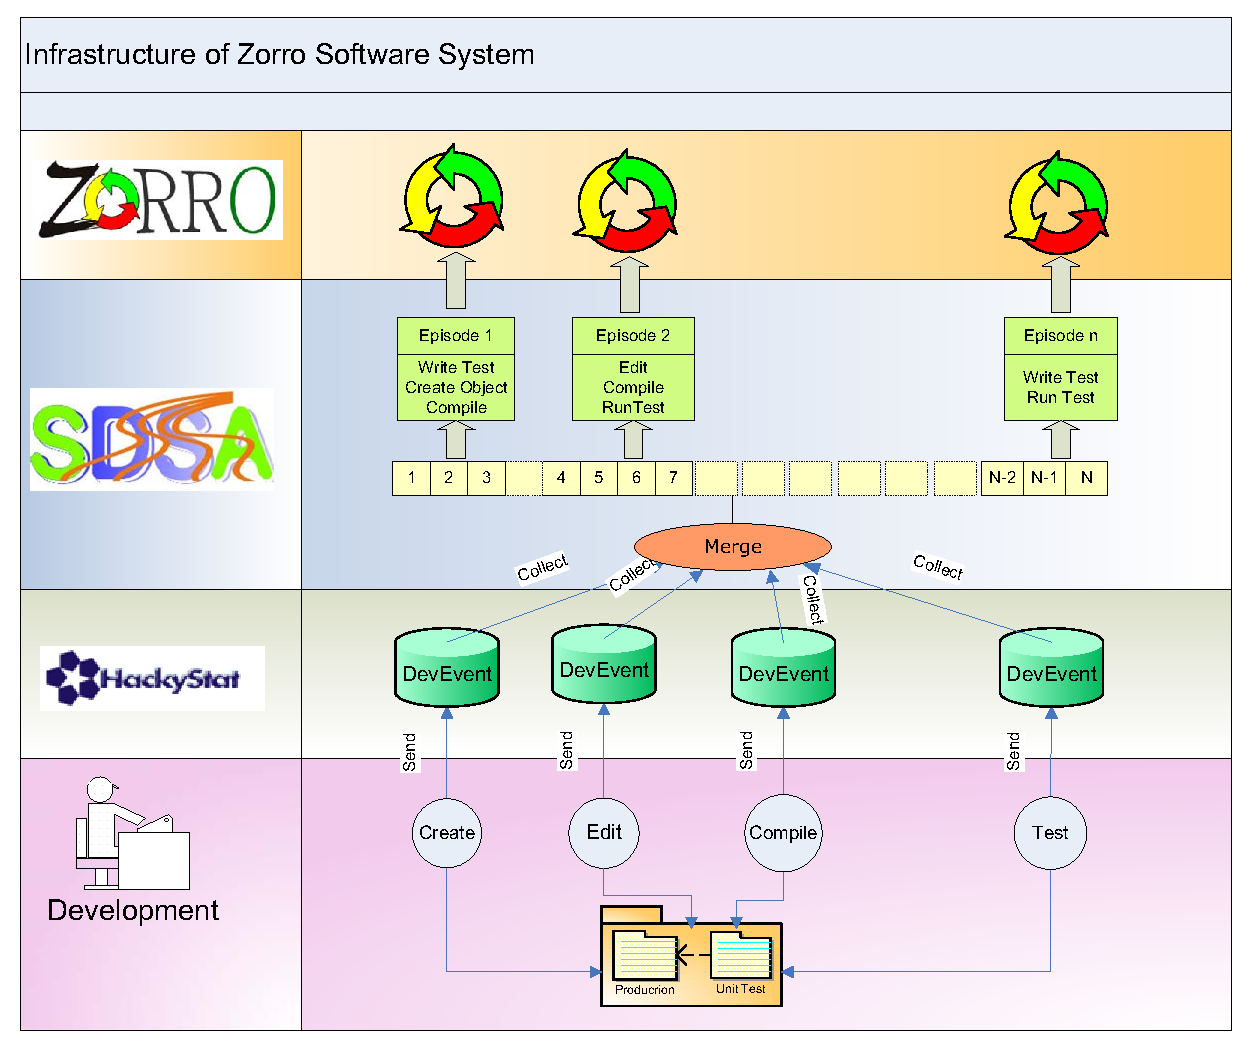
\includegraphics[width=0.9\textwidth]{figs/Zorro-Infrastructure.eps}
  \caption{Zorro Infrastructure}\label{fig:infra}
\end{figure}

With the capabilities provided by SDSA, I defined a set of specific rules
for TDD in Zorro according to Beck \cite{Beck:01,Beck:03} and others who have
described the practices of TDD. Zorro uses a two-step procedure to measure
and evaluate the compliance of the developer's behaviors with the practices
of TDD.  First, Zorro recognizes and classifies the episodes independently
according to the classification schema. Second, Zorro evaluates the
internal structure as well as the context of the episodes to deduce whether
an episode is TDD conformant or not.

















\chapter{Related Work}
\label{chap:RelatedWork}
Much of the research work on TDD suffers from the threat of ``construct
validity'' \cite{Wang:04} because of the what has been termed as the
``process conformance'' problem. Wang and Erdogmus defined process
conformance as the ability and willingness of the subjects to follow a
prescribed process.  Janzen warned that inability to accurately
characterize process conformance is harmful to TDD research
\cite{Janzen:05}: Many organizations might be using the methodology without
talking about it.  Others might claim to be using a methodology when in
fact they are misapplying it. Worse yet, they might be advertising its use
falsely.  Surveys might be conducted to gauge a method's usage, but often
only those who are much in favor or much opposed to the methodology will
respond.

A handful of research work has been done on software process validation
\cite{Cook:95,Jensen:05} and the process compliance of Test-Driven
Development \cite{csdl2-06-02,Wang:04,Wege:04}.  Cook and Wolf
\cite{Cook:95} developed a client-server software system called Balboa to
do process discovery and validation using a finite state machine (FSM).
Balboa collects developers' invocations of Unix commands and CVS commits to
learn the software process using FSM and machine learning techniques. Cook was 
able to reproduce the ISPW
6/7 process with Balboa in his research.  However, FSM does not look like
an ideal solution for process validation because of the complexity of the
process FSM it generates. In his example, the three algorithms RNET, KTAIL
and MARKOV generated 15, 20 and 25 states respectively, and the states are
interweaved in complicated manners. It is hard to interpret the process
state chart without thorough understanding of Balboa and the adopted
software process. Jansen and Scacchi \cite{Jensen:05} simulated an
automated approach to discovery and modeling of open source software
development processes.  They took advantage of prior knowledge to discover
the software development processes by modeling the process fragments using
a PML description. Their prototype simulation found that they could detect
unusually long activities and problematic cycles of activities. They
suggested that a bottom-up strategy, together with a top-down process
meta-modeling is suitable for automated process discovery. But they don't
have a working software system except for a prototype implementation.

Janzen \cite{Janzen:05} claimed that TDD is a kind of software development
method, not a process model, and that it has emerged out of a particular
set of process models. In contrast, Beck and Cunningham, the pioneers of
TDD, put it this way: ``test-first coding is not a testing technique but is
rather about design.''\cite{Beck:01} If TDD is a design technique and it
drives the implementation of product code, then classifying it as a
software process sounds reasonable. In my research, I have characterized
practices such as Test-Driven Development and Personal Software Process
(PSP) as low-level software processes. A common characteristic of a low-level
software process is that it is defined by many frequent and rapid
short-duration activities. Unlike high-level and long duration phases such
as ``requirement analysis'' that might last weeks to months, the activities
in low-level software process such as ``refactor class Foo to extract
interface IFoo'' may take only seconds to a few minutes \cite{csdl2-06-02}.

Low-level software processes often face similar research questions as
other, longer duration software processes. For instance, what process is
currently occurring, what process should occur, what are the impacts of a
given process on the important outcomes of software such as quality and
productivity, and how can a given process be improved and tailored in an
organization? So far, software engineering researchers have focused heavily
on the important outcomes that TDD brings to software products and software
developers. Both pedagogical
\cite{Muller:02,Edwards:04,Geras:04,Matjaz:03,Erdogmus:05,Kaufmann:03} and
industrial \cite{George:03,Maximilien:03,Bhat:06} evaluations of TDD have
been conducted in the last few years.  It is interesting to note that number of
research studies on TDD in academic settings is greater than the number of
research studies in industrial settings.

\section{Research Work in Academic Settings}
Most TDD research studies in academic settings seems to indicate that there
is some degree of quality improvement, but that there are little programmer
productivity benefits. Indeed, some studies have shown quality improvements
but at the cost of decreased productivity.

Muller and Hanger \cite{Muller:02} conducted a study in an XP class in
Germany to test TDD in isolation of other XP practices against traditional
programming.  The acceptance tests were provided to both the TDD group and
the control group. Interestingly, students in the TDD group spent more time
but their programs were less reliable than the control group.  

Edwards \cite{Edwards:04} adopted TDD in a junior-level class to compare
whether students got more reliable code after the use of TDD and WEB-CAT,
an assignment submission system. It turned out that the students using TDD
reduced their defect rate dramatically (45\% fewer defects/KSLOC using a
proxy metric) after adopting TDD, and a posttest survey found that TDD
students were more confident of the correctness and robustness of their
programs.

Geras, Smith and Miller \cite{Geras:04} also isolated TDD from other XP
practices, and investigated the impact of TDD on developer productivity and
software quality. In their research, TDD does not require more time but
developers in TDD group wrote more tests and executed them more frequently,
which may have led to future time savings on debugging and development.

Pancur \cite{Matjaz:03} designed a controlled experiment to compare TDD
with Iterative Test-Last approach (ITL), which is a slightly modified TDD
development process in the order of ``code-test-refactor''.  This study
found that TDD is somewhat different from ITL but the difference is very
small.

A more recent study on the effectiveness of TDD conducted by Erdogmus,
Morisio and Torchiano \cite{Erdogmus:05} used the well-defined test-last
and TDD approaches as Pancur did in \cite{Matjaz:03}. This study concluded
that TDD programmers wrote more tests per unit of programming effort. More
test code tends to increase software quality. Thus, TDD appears to improve
the quality of software but TDD group in the study did not achieve better
quality on average than test-last group.

Kaufmann \cite{Kaufmann:03}'s pilot study on implications of TDD, in
contrast, reported improved software quality and programmers' confidence.

\section{Research Work in Industrial Settings}
Several attempts have been made by researchers to study software quality
and productivity improvements of TDD in industrial settings.  

George and Williams \cite{George:04} ran a set of structured experiments
with 24 professional pair programmers in three companies. Each pair was
randomly assigned to a TDD group or a control group to develop a bowling
game application. The final projects were assessed at the end of the
experiment.  They found that TDD practice appears to yield code with
superior external code quality as measured by a set of blackbox test cases,
and TDD group passed 18\% more test cases. However, the TDD group spent
16\% more time on development, which could have indicated that achieving
higher quality requires some additional investment of time. Interestingly,
and in the contrast to the empirical findings, 78\% of the subjects
indicated that TDD practice would improve programmers' productivity.

Maximilien and Williams \cite{Maximilien:03} transitioned a software team
from an ad-hoc approach to testing to TDD unit testing practice at IBM, and
this team improved software quality by 50\% as measured by Functional
Verification Tests (FVT).

Another study of TDD at Microsoft conducted by Bhat and Nagappan
\cite{Bhat:06} reported remarkable software quality improvement as measured
in number of defects per KLOC. After introducing of TDD, project A
(Windows) reduced its defects rate by 2.6 times, and project B (MSN)
reduced its defect rate by 4.2 times, compared to the organizational
average. Reportedly, developers in project A spent 35\% more development
time, and developers in project B spent 15\% more development time, than
the developers in non-TDD projects spent.

\section{Process Conformance Study of TDD}
As we can see from the literature, there are discrepancies in the empirical
findings across both educational settings and industrial settings. Sometimes the
discrepancies are dramatic, for example \cite{Muller:02} found that the TDD
group yielded less reliable programs than the control group, while
\cite{Bhat:06} reported that the TDD group improved software quality by 
over four times.

Wang and Erdogmus \cite{Wang:04} pointed out there are several
possibilities that might explain why there are the discrepancies in TDD
research findings. For example, discrepancies could occur due to
differences in populations, differences in teaching methods and materials,
and differences in the techniques by which TDD is compared. They argued
that TDD empirical software research lacks process conformance, and
therefore it suffers from the construct validity problem (as is also the
case in some other empirical software engineering research). In
\cite{Wang:04}, they developed a prototype called TestFirstGauge to study
the process conformance of TDD by mining the in-process log data collected
by Hackystat. TestFirstGauge aggregates software development data collected
by Hackystat to derive programming cycles of TDD. They use T/P ratio (lines
of test code verse lines of production code), testing effort against
production effort and cycle time distribution as the indicator of TDD
process conformance. This project precedes the Zorro software system
\cite{csdl2-06-02}, and in fact it stimulated our research interest in
studying low-level software process conformance. Unlike the
prototype implementation of TestFirstGauge in VBA using an Excel
spreadsheet, Zorro is integrated into the Hackystat system for automation,
reuse, and flexibility using rule-based system \cite{Friedman-Hill:03}.

Similarly, Wege \cite{Wege:04} also focused on automated support of TDD
process assessment, but his work has a limitation in that it uses the CVS
history of code. Developers will not commit on-going project data at the
granularity of seconds, minutes or hours when they develop the software
system, making this data collection technique problematic for the purpose
of TDD inference.











\chapter{Research Questions}
\label{ch:researchquestions}
The long-term goal of my research is to understand how to characterize
and improve low-level software development behaviors.  As a step in
that direction, I am focusing for my Ph.D. research on a specific kind
of low-level software development behavior: Test-Driven
Development. The Zorro system, which attempts to infer TDD low-level
development behaviors, provides a way to partially evaluate the
overall approach and begin to understand its strengths and
limitations.

Zorro infers developer's TDD development behaviors using SDSA. It is
easy for software developers to collect in-process development
activities using Hackystat sensors, and it is also easy for them to
evaluate their TDD development behaviors using Zorro. If Zorro's TDD
inference is correct, then we can use it to assess TDD process
conformance during the daily practice of TDD as well as during empirical
studies of TDD. However, does Zorro infer developers' TDD development
behaviors correctly? Will it falsely categorize some non-TDD
development behaviors as TDD? Or, will it misinterpret some TDD
development behaviors as non-TDD? To answer these questions, we need 
to conduct validation studies of Zorro. Some of the most important research
questions are: 
\begin{itemize}
\item Q1: Can Zorro automate the recognition of Test-Driven Development
using automatically collected low-level software development activities?  
\item Q2: Can Zorro help to improve the practice of TDD? 

This is a hard question, but we can divide it into three small questions
with regard to user's roles.
   \begin{itemize}
   \item For beginners, can Zorro help them improve the compliance to TDD?
   \item For experienced TDD practitioners, will Zorro help them
   improve their TDD practice by analyzing their TDD development
   behaviors?
   \item For researchers, can Zorro help them reach legitimate
   research conclusions on TDD experiments by providing the TDD
   process conformance information.
   \end{itemize}
\end{itemize}

Answering these questions requires a ``mixed methods'' research strategy
\cite{Creswell:03}. Questions Q1 can be investigated by evaluating 
Zorro's data collection and TDD inference capability using field observation
research method. Investigating question Q2 requires research methods such  
as collecting users' feedback or interviewing them. In my research, 
I designed a series of case studies using these research methods to 
investigate the research questions I presented above.
\input{06-12-experiment-design.tex}
%\chapter{Data Analysis: Classroom Case Study}
\label{ch:ClassroomDataAnalysis}
The classroom case study is an evaluation designed to evaluate Zorro's
low-level development activity collection and automated inference
of Test-Driven Development behaviors. This chapter has three
sections. Section \ref{sec:CaseStudyMethod} explains the analysis
method for individuals using the first participant's data. Section
\ref{sec:CaseStudyFindings} presents the summary of analysis results
over all participants' data. In the end Section \ref{sec:discussion}
discusses the research findings from this research.

\section{Analysis Method for Individual}
\label{sec:CaseStudyMethod}

A participant in this study developed a solution to the Bowling Score
Keeper problem (Appendix \ref{app:UserStoriesBSK}) in the Eclipse IDE
with the instrumentations using the Hackystat Eclipse Sensor and
ESR. I collected both the participant's in-process development
activities and the participant's development video. During the data
analysis process, I played the ESR video to observe the participant's
development activities and TDD development behaviors. Then I compared
my observational results to the data that was automatically collected
and inferred by Zorro. Finally, I used the participant's comments on
his/her own TDD development behaviors as the second data source for
additional validation.

After the participant finished the programming task, I interviewed
him/her on unit testing and TDD. Then the participant evaluated
Zorro's usefulness. Thus, I had both the interview script and the
participant's evaluation of Zorro. I analyzed these two types of data
to investigate how useful Zorro is and how Zorro's analyses can be
used in the teaching and practices of Test-Driven Development.

This section starts with a discussion of the data analysis procedure,
followed by detailed analysis results and data interpretation.

\subsection{Data Analysis Procedure}

\begin{enumerate}
\item Observe development activities and partition development streams

Similarly to the pilot study, I observed low-level development activities
by playing the recorded ESR video. Then I logged them into an Excel 
spreadsheet. An activity has a start time, an end time, and a description 
as seen in Table \ref{fig:VideoExcel}. A participant's development stream 
is a sequential list of all the development activities that occurred in the 
participant's programming session in this study. In the end I divided the 
development stream into episodes as Zorro does after finishing the activity 
observation.

\item Validate Zorro using the the development video analysis

In this study, I designed user stories for the Bowling Score Keeper
problem (Appendix \ref{app:UserStoriesBSK}), which served as a TDD todo 
list. A participant typically solved a user story in one or more
episodes. While playing the participant's ESR video and observing his/her 
development activities, I also analyzed his/her TDD development behaviors. 
This technique is a variation of the participant observation for validating 
Zorro's automated TDD behavior inference machinery.

\item Cross-validate Zorro using the participant's comments

Although I tried hard to analyze the recorded ESR videos from a
nonpartisan point of view in the data analysis, it is possible that my
opinions are biased because I am also the developer of
Zorro. Therefore, I asked the participant to comment on his/her TDD
development behaviors after finishing the programming task. The
participant's comment provided me with additional information to
cross-validate Zorro's automated TDD behavior inference.

The participant commented on his/her TDD development behaviors by
answering the question -- ``Do you feel that this portion of
development is TDD?''  and checking the following items that could be
applied: ``adding new functionality'', ``refactoring'', ``adding
test'', ``just running tests'', ``can't tell'' and ``other''. For the
data analysis, I compared the participant's comments to Zorro's
inferences to investigate how accurately Zorro can infer TDD behaviors
in his/her opinion.

\item Analyze the Participant Interview using the Coding Method

The red/green/refactor metaphor is a simple and abbreviated
abstraction of TDD. A developer may conduct TDD development
differently depending upon his/her programming experiences and
understandings of TDD. Sometimes a developer may choose to violate
the principles of TDD intentionally. In this study, I interviewed
the participant on unit testing and TDD. Based on his/her answers 
to the interview questions, I coded him/her into different categories 
with the hope that the categorization of participants could be helpful in
interpreting the research findings from this study. The coding method
is a classical data analytical technique that has been widely adopted
by the qualitative research methods \cite{Creswell:03,GroundedTheory}.

\item Report the participant's usefulness evaluation

The participant reviewed the 5 analyses of Zorro to analyze his/her
TDD development behaviors in this study. I reported the participant's
evaluation regarding the usefulness of Zorro.

\end{enumerate}

In the rest of this section, with the first participant's data as an
example, I will present the individual data analysis results.

\subsection{Observation of development activities}
\label{subsec:DevelopmentActivityObservation}

\subsubsection{Analysis Result}
The first participant finished 7 of 13 user stories in 90
minutes. According to my observation, this developer conducted 153
development activities, and I divided them into 10 episodes. Table
\ref{tab:ActivityNumber} lists the number of activities collected 
and the number of activities I observed in each episode. The
difference between the two numbers lies in the ``Difference'' column. 
The statistics analysis results are at the end of this table in 
which ``STDEV'' standards for standard deviation.
\begin{table}[!h]
\centering
  \begin{tabular}{|l|l|l|l|}
  \hline
    Episode &  Activities (Zorro)& Activities (Video) & Difference \\ \hline
    1	      &   4 &   4  &   0   \\ \hline
    2	      &   6 &   5  &  +1   \\ \hline
    3       &  13 &  11  &  +2   \\ \hline
    4       &  19 &  15  &  +4   \\ \hline
    5       &  23 &  19  &  +4   \\ \hline
    6       &  14 &   9  &  +5   \\ \hline
    7       &  46 &  35  &  +11  \\ \hline
    8       &  22 &  15  &  +7   \\ \hline
    9       &   5 &   5  &   0   \\ \hline
    10      &  46 &  35  &  +11  \\ \hline \hline
    Total   & 198 & 153  &       \\ \hline
    Average &     &      &  4.5  \\ \hline
    Median  &     &      &  4    \\ \hline
    STDEV   &     &      &  4.1  \\ \hline
    \end{tabular}
  \caption{Number of Development Activities}\label{tab:ActivityNumber}  
\end{table}

\subsubsection{Data Interpretation}

Table \ref{tab:ActivityNumber} tells us that activities collected
by Zorro outnumbered activities I observed in the recorded ESR
video. The fact that ESR captures the Eclipse screen once per second
determines that it can capture almost everything that happens in a
software programming session, but Zorro can collect either equal or 
even more amount of development activities for the first participant. 
Zorro collected 4.5 more activities per episode than I observed in 
the video on average. The standard deviation is 
\begin{equation} \label{StandardDeviation}
  s = \sqrt{\frac{\sum_{i=1}^{10}{(x_{i}-\bar{x})^2}}{n-1}} = 4.1.
\end{equation},
where \begin{math}s\end{math} standards for standard deviation, 
\begin{math}x_{i}\end{math} standards for the activity number difference 
of the \begin{math}ith\end{math} episode, and \begin{math}\bar{x}\end{math} 
is the mean of episode activity differences.

\subsection{Validation of Zorro using video analysis}

\subsubsection{Analysis Result}
Table \ref{tab:BehaviorObservation} lists the development behavior
and TDD compliance of each episode. The Zorro's inference results 
are on the left and my video observation results are on the right in 
Table \ref{tab:BehaviorObservation}. 

\begin{table}[!htbp]
\centering
  \begin{tabular}{|l|p{2cm}|l|p{2cm}|l|}
  \hline
         & \multicolumn{2}{c|}{Zorro} & 
           \multicolumn{2}{c|}{Video Observation} \\ \cline{2-5}
   \raisebox{1.5ex}[0pt]{Index} 
         & Behavior       & Is TDD? & Behavior      & Is TDD? \\ \hline
    1    & test-addition  & Yes	    & test-addition & Yes   \\ \hline
    2    & refactoring	  & Yes	    & refactoring   & Yes   \\ \hline
    3    & refactoring	  & Yes	    & refactoring   & Yes   \\ \hline
    4    & test-first     & Yes     & test-first    & Yes   \\ \hline
    5    & test-first     & Yes     & test-first    & Yes   \\ \hline
    6    & test-first     & Yes	    & test-first    & Yes  \\ \hline
    7    & test-first     & Yes	    & test-first    & Yes  \\ \hline
    8    & test-first     & Yes     & test-first    & Yes   \\ \hline
    9    & test-addition  & Yes	    & test-addition	& Yes	 \\ \hline
   10    & unknown        & No      & test-first    & Yes  \\ \hline 
  \end{tabular}
  \caption{Comparison between Zorro Inference and Video Observation}\label{tab:BehaviorObservation}  
\end{table}

\subsubsection{Data Interpretation}

My video observation results on development behaviors and TDD compliance
are identical to Zorro's inference results. Note that the last
episode is exceptional because it is incomplete. The first participant
spent more than 40 minutes on the last user story but did not finish it
because of the time constraint. Zorro can not infer the development
behavior in the last episode because it does not end with successful 
unit test runs, which is an implicit protocol of the Zorro software 
system. 

\begin{comment}
Because the last episode was 
incomplete, Zorro did not recognize what happened in it. Other than this, 
the results inferred by Zorro and the results observed by me are
identical.

The data in Table \ref{tab:BehaviorObservation} provide complementary
evidence to the research finding in Section
\ref{subsec:DevelopmentActivityObservation} for the research question
Q2a. All episodes were partitioned and the development behaviors in
them were inferred correctly by Zorro if the last episode was not
considered.
\end{comment}

\subsection{Cross-validation of Zorro using participant comment analysis}

\subsubsection{Analysis Results}
As the developer of Zorro, my video observation could be biased if it were
the only validation method. The participant comments provided the additional 
data source to cross-validate Zorro's automated TDD behavior inference. 
For this purpose, in Table \ref{tab:ParticipantTDDBehavior}, I list the first
participant's comments along with both Zorro's inference results and my
video observation results. Note that the participant's comments on 
development behaviors are different from what Zorro inferred and I 
observed in the ESR video. In this study, the participants commented their 
development behaviors by selecting any inclusive development behaviors from 
the following list: 
\begin{itemize}
\item adding new functionality,
\item refactoring,
\item adding test,
\item just running tests,
\item can't tell,
\item other
\end{itemize}
for each episode. Both Zorro and my video observation categorized the
development behavior in each episode using the tacit knowledge of the
TDD development patterns.

\begin{sidewaystable}[!htbp]
\centering
  \begin{tabular}{|l|p{2cm}|l|p{2cm}|l|p{7.5cm}|l|}
  \hline
      & \multicolumn{2}{c|}{Zorro Inference} & \multicolumn{2}{c|}{Video Observation} & 
        \multicolumn{2}{c|}{Participant Comment} \\ \cline{2-7}
   \raisebox{1.5ex}[0pt]{Index} &
    Behavior      & Is TDD? & Behavior  & Is TDD? & Behavior & Is TDD? \\ \hline
1 & test-addition & Yes & test-addition & Yes & adding test  & Yes \\ \hline
2 & refactoring   & Yes & test-first    & Yes & refactoring & Yes  \\ \hline
3 & refactoring   & Yes & refactoring   & Yes & refactoring & Yes  \\ \hline
4 & test-first    & Yes & test-first    & Yes & adding new functionality, adding test & Yes	\\ \hline
5 & test-first    & Yes & test-first    & Yes & refactoring & Yes  \\ \hline
6 & test-first    & Yes & test-first    & Yes & adding new functionality, adding test & Yes \\ \hline
7 & test-first    & Yes & test-first    & Yes & adding new functionality, refactoring, adding test & Yes \\ \hline
8 & test-first    & Yes & test-first    & Yes & adding new functionality, adding test & Yes	\\ \hline
9 & test-addition & Yes & test-addition & Yes & adding test & Yes  \\ \hline
10 & unknown      & No  & test-first    & Yes & adding new functionality, refactoring, adding test & Yes \\ \hline 
  \end{tabular}
  \caption{Participants' Comments on their Development Behaviors}
  \label{tab:ParticipantTDDBehavior}  
\end{sidewaystable}

\subsubsection{Data Interpretation}

The first participant believed that his development process was 100\%
TDD compliant, which is slightly different from what Zorro inferred
but conformant to what I observed in the video. The cause of this
difference is due to Zorro's stringent requirement that an episode
must end with successful unit test invocations. 

In term of the development behavior, it is not possible to directly
compare the development behaviors commented by the participant with
what Zorro inferred and I observed. I will introduce a mapping schema
to make them comparable in the next section.

\begin{comment}
Although the terms for describing episode behaviors were different,
the participant's comments provided enough information to validate
Zorro's episode behavior inference. For example, the first participant
agreed that Zorro correctly inferred the behaviors in episodes 1, 2,
3, and 9. Episodes 4, 6, 7, and 9 are ``test-driven'' with compound
development behaviors from the participant's points of view. 

Most importantly, the participant's comments provided the additional
information to cross-validate the video analysis method. For the first
participant, his comments were very close to what I have observed
using the video analysis. 
\end{comment}

\subsection{Interview questions and responses}

\subsubsection{Analysis Results}

Table \ref{tab:InterviewQuestionAndAnswer} lists the interview questions 
and the first participant's responses. The first column has the brief 
summaries of interview questions. The second column includes the coding 
results of the participant's answers.

\begin{table}[!h]
\centering
  \begin{tabular}{|l|p{8cm}|}
  \hline
    Interview Question & Participant's Response \\ \hline
    Unit testing experience         & Several years.\\ \hline
    Prior unit testing strategy     & Write test after production iteratively.\\ \hline
    How much unit testing           & Not all the time. \\ \hline
    TDD's impact on unit testing    & TDD is messy and leads to wrong design. 
                                      TDD is better if there is good design first. \\ \hline
    Comfortableness of TDD          & Hard, especially when a refactoring activity  
                                      caused previous tests failed (regression test failure). 
                                      \\ \hline
    Full-scale use of TDD           & Do not want to do so until I get accustomed 
                                      to it. Likes the idea of TDD.\\ \hline
  \end{tabular}
  \caption{List of Interview Questions and Answers}\label{tab:InterviewQuestionAndAnswer}  
\end{table}

\subsubsection{Data Interpretation}
 
The first participant is ``somewhat in favor of unit testing but not in 
favor of TDD'' according to his answers. Unit testing
was a practice that was demanded in his prior software development. In his
opinion, iteratively implementing test cases afterward makes more sense than 
TDD.  Additionally, TDD may lead to wrong design and messy code if there is no
good design first. Therefore, implementing software in TDD is hard and it 
takes time to get accustomed to TDD. So I put him in the category 
of ``somewhat in favor of unit testing but not in favor of TDD''.
Moreover, his answers reflected what had happened in the last episode, in 
which the revised production code failed some regression tests and he 
could not make all tests pass at the end. 

\subsection{Usefulness evaluation}

While evaluating Zorro's usefulness, the first participant also
expressed how strongly he agreed that Zorro's analyses were
useful. The strengthen of usefulness varies from ``Strongly Agree'' to
``Strongly Disagree'', which are quantified to values 5 to 1 (Table
\ref{tab:UsefulnessScale}).
\begin{table}[!h]
\centering
  \begin{tabular}{|l|l|}
  \hline
   Strengthen        & Scale \\ \hline
   Strongly Agree    & 5 \\ \hline
   Agree             & 4 \\ \hline
   Neutral           & 3 \\ \hline
   Disagree          & 2 \\ \hline
   Strongly Disagree & 1 \\ \hline
  \end{tabular}
  \caption{Table of Usefulness Scale}\label{tab:UsefulnessScale}  
\end{table}

Moreover, the first participant checked which areas were helpful to
him after reviewing his development processes using Zorro's
analyses. Table \ref{tab:UsefulAreas} is a list of all possible useful
areas that are encoded to UA-1, UA-2, and UA-3 etc.
\begin{table}[!h]
  \centering
  \begin{tabular}{|l|l|}
  \hline
  Code & Useful Area \\ \hline
  UA-1 & Acquiring awareness of my programming patterns \\ \hline
  UA-2 & Learning TDD \\ \hline
  UA-3 & Mastering TDD \\ \hline
  UA-4 & Monitoring my pace \\ \hline
  UA-5 & Improving my programming skills \\ \hline
  UA-6 & Discovering the situations in which TDD is useful \\ \hline
  UA-7 & Discovering the situations in which TDD is applicable \\ \hline
  UA-8 & Gauging how much testing I am doing \\ \hline
  UA-9 & Other \\ \hline
  \end{tabular}
  \caption{Table of Useful Areas}\label{tab:UsefulAreas}  
\end{table}

\subsubsection{Analysis Results}

Table \ref{tab:FirstUsefulness} is a summary of the first participant's 
evaluation on Zorro's usefulness. He evaluated 4 of Zorro's 5 analyses,  
but the analysis ``Effort T/P Ratio'', which had a bug at that time. 
I fixed it later on for the rest of participants.
\begin{table}[!ht]
\centering
  \begin{tabular}{|l|l|l|l|l|l|l|l|l|l|l|}
  \hline
           &      & \multicolumn{9}{c|}{Areas} \\ \cline{3-11}
    \raisebox{1.5ex}[0pt]{Analysis Name}   & \raisebox{1.5ex}[0pt]{Scale} 
       & UA-1 & UA-2 & UA-3 & UA-4 & UA-5 & UA-6 & UA-7 & UA-8 & UA-9   \\ \hline
    Demography Analysis & 3   &   & X &   &   & X &   & X &   &   \\ \hline       
    Effort T/P Ratio    & N/A &   &   &   &   &   &   &   &   &   \\ \hline
    Size T/P Ratio      & 2   &   &   &   & X &   &   &   &   &   \\ \hline
    Duration            & 3   &   &   &   & X &   &   &   &   &   \\ \hline
    Duration Histogram  & 2   &   &   &   & X &   &   &   &   &   \\ \hline
  \end{tabular}
  \caption{The First Participant's Usefulness Evaluation}\label{tab:FirstUsefulness}
\end{table}


\subsubsection{Data Interpretation}

The first participant thought that Zorro's analyses were somewhat useful 
to him. The average usefulness strength is 3.5 basing on the values listed in 
Table \ref{tab:UsefulnessScale}. According to him the analysis analysis 
``TDD Episode Demography'' was the most useful one for learning TDD 
whereas other analyses were just good at showing his development pace. 

\section{Summary of Data Analysis Results}
\label{sec:CaseStudyFindings}
Eleven students from the software engineering classes in Fall 2006
participated in this study. I assigned letters 'A', 'K', 'L',
'M', 'N', 'O', 'P', 'Q', 'R', 'S', and 'T' to them as their identifications.
I will show the data analysis results, and discuss the research 
findings out of this research in this section.

Before presenting data analysis results, I will introduce an unexpected
phenomenon I discovered in the data analysis process, which had
negative impacts on Zorro's development stream partition and TDD
behavior inference. 

\subsection{An unexpected phenomenon and participant grouping}
\label{subsec:ParticipantGroup}

In Chapter \ref{chap:intro}, we have discussed that the software 
development of TDD is iterative and incremental. According to Kent 
Beck\cite{Beck:03}, the rhythm of TDD is:
\begin{enumerate}
\item Quickly add a test.
\item Run all the tests and see the new one fail.
\item Make a little change.
\item Run all tests and see them all succeed.
\item Refactor to remove duplication.
\end{enumerate}

Based on the rhythm of TDD, I designed Zorro to partition a developer's
TDD development stream over a time period into episodes using successful
test invocations as tokens. Through literature readings, my personal 
practices, and observation of others programming in TDD, this partition
technique should work very well toward recognizing the TDD practices.

However, an unexpected phenomenon I found in my video observation 
diverted Zorro's partition of software development streams. 
Note that step 2 of the TDD rhythm is to ``run all the tests and see 
the new one fail''. But the test invocation can surprisingly succeed 
when the test code has compilation errors. In this case, the Eclipse
would prompt with an alert message saying that there is compilation 
errors and giving the developer options to either continue or cancel 
the test invocation. The test invocation may succeed if the developer 
chooses to continue it regardless of compilation errors. If it succeeds, 
Zorro could wrongly partition the development stream in the middle of 
a TDD iteration, which would, in turn, lead to partition and inference 
errors.

To investigate how this phenomenon affected Zorro, I divided the 
participants into groups G1 and G2 based upon their test invocation
behaviors.
\begin{itemize}
\item \textbf{G1} Participants who halted a test invocation when there were compilation errors.
\item \textbf{G2} Participants who continued a test invocation regardless of compilation errors.
\end{itemize}
Among 11 participants, 4 of them are in group G1 and 7 of them are in group 
G2 (see Table \ref{tab:ParticipantCategory}).  
\begin{table}[!ht]
\centering
  \begin{tabular}{|l|l|l|l|}
  \hline
    Group &  Participants \\ \hline
    G1	     &  K, L, O, and R \\ \hline
    G2	     &  A, M, N, P, Q, S, and T  \\ \hline
    \end{tabular}
  \caption{Participant Groups}\label{tab:ParticipantCategory}  
\end{table}

Since the partition and inference errors can only occur for 
participants in group G2, I would term this development behavior
as G2-DevBehavior in the rest of this document.

\subsection{Validation of development activities}
\label{subsec:SensorDataValidation}
I observed all participants' development activities using the recorded ESR
videos, and compared the observed activities to the activities collected
by Zorro for validation. 

\subsubsection{Analysis Result}
Table \ref{tab:ActivityNumberSummary} presents numbers of development
activities for each participant. The first column includes the participant 
IDs. The second column has the number of episodes that were partitioned
by Zorro. For each participant, I listed development activities per episode
in columns 3 and 4. The number of activities collected by Zorro is in 
column 3 and the number of activities I observed in the video is in column 
4. The rest two columns have the mean and median values of episode activity 
number differences.

\begin{table}[!ht]
\centering
  \begin{tabular}{|l|r|r|r|r|r|}
  \hline
    &  &  \multicolumn{2}{c|}{Activities per Episode} & 
          \multicolumn{2}{c|}{Activity Difference} \\ \cline{3-6}
    \raisebox{1.5ex}[0pt]{ID} & \raisebox{1.5ex}[0pt]{Episodes}  & 
                 Zorro & Video Observation & Average & Median \\ \hline
         A  & 19   & 12.7 & 11.9 & 0.8 & 0   \\ \hline  
         K  & 10   & 19.8 & 15.3 & 4.5 & 4   \\ \hline
         L  &  8   & 32.5 & 30.4 & 2.1 & 2   \\ \hline  
         N  &  9   & 20.4 & 18.2 & 2.2 & 3   \\ \hline
         O  & 16   & 15.3 & 13.6 & 1.7 & 0.5 \\ \hline
         P  & 18   & 13.7 & 11.7 & 2.1 & 1.5 \\ \hline
         Q  & 21   &  9.8 &  9.6 & 0.5 & 0   \\ \hline
         R  & 14   & 12.6 & 11.2 & 1.4 & 0   \\ \hline
         S  &  9   & 16.3 & 12.7 & 3.7 & 2   \\ \hline
         T  & 13   & 15.3 & 13.2 & 2.1 & 1   \\ \hline
    Average & 13.8 & 16.8 & 14.8 & 2.1 & 1.4 \\ \hline 
    \end{tabular}
  \caption{Summary of Development Activities}\label{tab:ActivityNumberSummary} 
\end{table}

Note that I excluded the data from participant 'M' in Table \ref{tab:ActivityNumberSummary},
which helped me find a bug in the Eclipse sensor. The bug is related to
the unexpected phenomenon I discussed in Section \ref{subsec:ParticipantGroup}.
There was an unhandled exception when the participant 'M' forced Eclipse
to launch the tests regardless of compilation errors. As a consequence, the 
sensor missed some unit test invocations. I fixed this bug after
finding it, but Zorro can not partition his development stream correctly 
due to the loss of test invocation data. Fortunately, this bug fix helped 
me avoid data loss for the rest participants. 

\subsubsection{Discussion}
According to Table \ref{tab:ActivityNumberSummary}, Zorro is capable of
collecting development activities. The Zorro sensor collected more 
development activities (16.8 per episode) than what I observed in the
recorded ESR videos (14.8 per episode). Both the mean and median values
of episode activity number differences are bigger than or equal to zero.  

I did further investigation to find the causes to the activity number 
differences by comparing the development activities collected by Zorro 
with the development activities I observed in the recorded ESR videos
(Figure \ref{fig:ZorroDataValidation}). 
\begin{figure}[!h]
  \centering
  \includegraphics[width=1.0\textwidth]{figs/ZorroSensorDataValidation.eps}
  \caption{Validation of Zorro's Development Activities}
  \label{fig:ZorroDataValidation}
\end{figure}

With side by side comparison, I found two reasons for the activity number
differences. First, Zorro can collect two activities for one 
development behavior. Nearly 100\% of development behaviors I observed 
in ESR videos could be found in Zorro, but the relationship was not always 
one-to-one. Sometimes Zorro reported two or more activities for one observable 
development behavior in an ESR video as I described 
in item ``Kill two birds with one stone''. Second, although the ESR should 
capture everything that happens in the Eclipse IDE, it still has its 
limitations. I addressed them in items ``Invisible editing activities'' 
and ``Problem view of Eclipse could be hidden''.
\begin{enumerate}
  \item Kill two birds with one stone
  
  When a developer changed statements that were associated with object
  components such as import, package declaration, field variables, and
  method name, return type, or parameters, the Zorro sensor would
  collect two types of development activities: editing and
  refactoring. Similarly the Zorro sensor would collect both types
  of development activities when a developer used the refactoring
  commands supplied in Eclipse. This item contributed most to the
  differences of episode activity numbers.

  \item The problems view of Eclipse was hidden
  
  The problems view of Eclipse was overlapped by other views for a
  while (see Figure \ref{fig:InvisibleEclipseProblemView}) in the ESR
  videos of participants K, M, and T. Since Eclipse reports compilation
  errors in the problems view, I could not observe compilation errors in
  the ESR videos in this situation. For instance, in Figure
  \ref{fig:InvisibleEclipseProblemView}, the JavaDoc view overlapped
  the problems view.  Since the title of the problems view was highlighted, 
  it probably meant that there should have had compilation errors, but I could 
  not tell it by watching the ESR video. 
  \begin{figure}[htbp]
    \centering
    \includegraphics[width=0.8\textwidth]{figs/ESR-InvisibleProblemPane.eps}
    \caption{Invisible Problem View in Eclipse}
    \label{fig:InvisibleEclipseProblemView}
  \end{figure}  

  \item Invisible editing activities

  A developer could input a few blank spaces while programming. Since
  ESR captured the screen of Eclipse, I would not be able to observe
  this kind of development activities because there is no visible 
  changes. 

\end{enumerate}

The above three items can answer why Zorro collected more development 
activities than what I observed in the videos. However, there
were also a few cases in which Zorro missed development activities (see 
items ``Quick editing'' and ``Quick buffer transition'').
\begin{enumerate}
 
  \item Quick editing
  
  The Zorro sensor uses ``state change'' as the foundation to detect
  editing development activities. A timer thread in the sensor wakes up every 10
  seconds to check the active buffer. If there are any changes made to
  the active buffer, the sensor will fire a ``state change'' event. Zorro
  reduces a series of consecutive ``state change'' events into an
  editing activity when processing development streams. This
  mechanism works well unless a developer edits a file for
  less than 10 seconds and then switches to another buffer. If so, the
  Zorro sensor will miss an editing development activity.

  \item Quick buffer transition
  
  The Zorro sensor collects ``buff trans'' activities by checking the
  active buffer.  A timer thread wakes up every 5 seconds to detect
  whether there is a buffer transition activity. Five-second is a
  small time period, but it is long enough for a developer to change
  the active buffers two or more times. If two or more consecutive buffer
  transition activities occur in less than 5 seconds, the Zorro sensor
  might fail to capture some or all of them.
   
\end{enumerate}        

\subsubsection{Conclusion}
In this section, I compared development activities collected by
Zorro with development activities I observed in the recorded 
development videos (see Table \ref{tab:ActivityNumberSummary}). 
Both the mean and median values of episode activity number differences 
are bigger than or equal to zero. Zorro collected more development 
activities than what I observed in the videos for every participant. 
There is partial evidence to support the research question Q2a 
(Chapter \ref{ch:ExperimentDesign}) from the data analysis in 
this section: Zorro can collect development activities more 
precisely than the video observation method.

\subsection{Validation using video observation}
\label{subsec:VideoObservationValidation}
Zorro recognizes TDD development through two steps: (1) inferring 
episode behaviors by matching development activities in episodes 
partitioned from development streams to a set of predefined 
development behaviors; (2) and then deducing the TDD compliance 
using the inferred episode behaviors. Thus, the video observation
validation process also has two steps: episode behavior validation
and TDD compliance validation.

When observing participants' development process videos, I analyzed
both their episode behaviors and TDD compliance. 
Table \ref{tab:BehaviorObservation} is an example of the analyzed 
results for one participant. I used my analyzed results to 
validate Zorro after I had observed the videos from all participants.

\subsubsection{Validation of Episode Behavior Inference}
\label{subsubsec:EpisodeBehavior}
I compared the episode behavior in each episode for every participant.
If my video observation analysis on the behavior in an episode agreed with 
what Zorro inferred, I assigned the boolean value 1 to this 
episode. Otherwise, I assigned value 0 to the episode. In the end, I 
added up all the 1's episodes. Table \ref{tab:EpisodeBehaviorAgreed} 
lists the number of total episodes, number of 1's episodes, and percent 
of 1's episodes for each participant. 
\begin{table}[!ht]
\centering
  \begin{tabular}{|l|r|r|r|}
  \hline
    ID & Episodes  & 1's Episodes & Percent of 1's Episodes\\ \hline
    A       & 19   &  15   & 78.9\% \\ \hline  
    K       & 10   &   8   & 80.0\% \\ \hline
    L       &  8   &   7   & 87.5\% \\ \hline  
    N       &  9   &   4   & 44.4\% \\ \hline
    O       & 16   &  15   & 93.8\% \\ \hline
    P       & 18   &  12   & 66.7\% \\ \hline
    Q       & 21   &  11   & 52.4\% \\ \hline
    R       & 14   &  13   & 92.9\% \\ \hline
    S       &  9   &   2   & 22.2\% \\ \hline
    T       & 13   &   9   & 69.2\% \\ \hline
    Total   & 137  &  96   & 70.1\% \\ \hline
    \end{tabular}
  \caption{Video observation validation of episode behaviors}
  \label{tab:EpisodeBehaviorAgreed} 
\end{table}

From Table \ref{tab:EpisodeBehaviorAgreed}, we can see that Zorro's 
episode behavior inference accuracy fluctuates from participant to 
participant. The lowest percentage is only 22.2\% and the highest
percentage is up to 93.8\%. Out of the 137 total episode behaviors, 
96 were inferred by Zorro correctly according to my video observation
analysis validation.

In Section \ref{subsec:ParticipantGroup}, we discussed that the
G2-DevBehavior had caused episode partition and inference errors for
participants in group G2. Now that Zorro's episode behavior inference
accuracy fluctuates, I am going to separate the participants of
this study using the G2-DevBehavior. Table \ref{tab:EpisodeBehaviorAgreedG1} 
lists the validation results of episode behaviors for participants 
in group G1. Table \ref{tab:EpisodeBehaviorAgreedG2} lists 
the validation results of episode behaviors for participants in
group G2.
\begin{table}[!ht]
\centering
  \begin{tabular}{|l|r|r|r|}
  \hline
    ID & Episodes  & 1's Episodes & Percent \\ \hline
    K       & 10   &   8   &  80.0\%  \\ \hline
    L       &  8   &   7   &  87.5\%  \\ \hline  
    O       & 16   &  15   &  93.8\%  \\ \hline
    R       & 14   &  13   &  92.9\%  \\ \hline
    Total   & 48   &  43   &  89.6\%  \\ \hline
    \end{tabular}
  \caption{Video observation validation of episode behaviors for G1 participants}
  \label{tab:EpisodeBehaviorAgreedG1} 
\end{table}
\begin{table}[!ht]
\centering
  \begin{tabular}{|l|r|r|r|r|}
  \hline
    ID & Episodes  & 1's Episodes & Percent & Episodes with G2-DevBehavior\\ \hline
    A       & 19   &  15   &  78.9\%  & 3  \\ \hline  
    N       &  9   &   4   &  44.4\%  & 3  \\ \hline
    P       & 18   &  12   &  66.7\%  & 4  \\ \hline
    Q       & 21   &  11   &  52.4\%  & 9  \\ \hline
    S       &  9   &   2   &  22.2\%  & 2  \\ \hline
    T       & 13   &   9   &  69.2\%  & 3  \\ \hline
    Total   & 89   &  53   &  59.6\%  & 24 \\ \hline
    \end{tabular}
  \caption{Video observation validation of episode behaviors for G2 participants}
  \label{tab:EpisodeBehaviorAgreedG2} 
\end{table}
The inference accuracy is 89.6\% for group G1 participants, but it 
is only 59.6\% for group G2 participants. In the best case, Zorro 
inferred 78.9\% of episode behaviors correctly for group G2 participants;
on the contrary, even the lowest inference accuracy for group G1
participants is already 80.0\%. Of 89 episodes in 
Table \ref{tab:EpisodeBehaviorAgreedG2}, 24 were affected by the 
G2-DevBehavior. So it had great impacts on Zorro's development 
stream partition and episode behavior inference.

\subsubsection{Validation of TDD Compliance Inference}
Zorro partitions a participant's development stream into episodes and
infers the TDD compliance of those episodes. An episode is TDD
compliant if its development behavior is either a portion of a
TDD iteration, such as refactoring, or a complete TDD iteration. 
Beyond validating episode behavior inference, I also validated
Zorro's TDD compliance inference. Table \ref{tab:TDDCompliantEpisodeNumber} 
lists the validation results. In the ``TDD Compliant Episodes''
columns, I include the number of TDD compliant episodes inferred 
by Zorro, the number of TDD compliant episodes I observed in the
videos, and the difference between them for each participant. 
\begin{table}[!ht]
\centering
  \begin{tabular}{|l|r|r|r|r|}
  \hline
    &  &  \multicolumn{3}{c|}{TDD Compliant Episodes} \\ \cline{3-5}
    \raisebox{1.5ex}[0pt]{ID} & \raisebox{1.5ex}[0pt]{Episodes}  & 
     By Zorro &  By Video Analysis & Difference\\ \hline
    A       &  19   &  10    &  12  & -2  \\ \hline  
    K       &  10   &   9    &  10  & -1  \\ \hline
    L       &   8   &   7    &   7  &  0  \\ \hline  
    N       &   9   &   6    &   8  & -2  \\ \hline
    O       &  16   &  15    &  16  & -1  \\ \hline
    P       &  18   &  16    &  18  & -2  \\ \hline
    Q       &  21   &  21    &  21  &  0  \\ \hline
    R       &  14   &  13    &  14  & -1  \\ \hline
    S       &   9   &   3    &   9  & -6  \\ \hline
    T       &  13   &  13    &  13  &  0  \\ \hline
    Total   & 137   & 113    & 128  & -15 \\ \hline
    Mean    &      &        & 	& -1.5 \\ \hline
    Median  &      &        & 	& -1  \\ \hline
    STDEV   &      &        & 	& 1.78 \\ \hline
    \end{tabular}
  \caption{Video observation validation of TDD compliance}
  \label{tab:TDDCompliantEpisodeNumber} 
\end{table}
Zorro inferred that the overall TDD compliance of this study was 
\[
   TDD(Zorro)\% = \frac{CompliantEpisodes(Zorro)}{TotalEpisodes} * 100
   = \frac{113}{137} * 100 = 82.5.
\]
In contrast, my video observation analysis concluded that 
\[
   TDD(Video Analysis)\% =
   \frac{CompliantEpisodes(VideoAnalysis)}{TotalEpisodes} * 100 =
   \frac{128}{137} * 100 = 93.4
\]
of episodes were TDD compliant. So, according to my video observation
analysis, Zorro is somewhat conservative on TDD compliance inference.  

From Table \ref{tab:TDDCompliantEpisodeNumber}, we can see that
the difference of TDD compliant episodes is either equal to or less 
than 0 for every participant. The mean value is -1.5 with 
standard deviation 1.78. Thus, the Zorro's TDD compliance inference
is very close to my video observation analysis.

In order to get a sense of how the Zorro's inference results fit the
video observation results, I will run the Chi-Square goodness-of-fit 
test. The goodness-of-fit test is to test whether a given distribution 
fits a set of data by comparing an observed frequency with the hypothesized 
distribution \cite{GoodnessOfFit,Anderson:86}. Letting \begin{math}p_{1},
p_{2}, ..., p_{10} \end{math} denote the percentages of TDD compliant 
episodes for participants inferred by Zorro, the null hypothesis 
would be
\[
    H: p_{1} \neq p_{10},p_{2} \neq p_{20}, ..., p_{10} \neq p_{100}, 
\]
where \begin{math}p_{10},p_{20}, ..., p_{100} \end{math} are the
percentages of TDD compliant episodes I observed in the process
videos. If Zorro inferred TDD compliance accurately, we will reject
the null hypothesis.

Let \begin{math}E_{i}\end{math} denote the expected number of TDD
compliant episodes for the \textit{ith} participant and
\begin{math}O_{i}\end{math} denote the number of TDD compliant 
episodes inferred by Zorro. The Chi-Square test is
\begin{equation} \label{ChiEquation}
  \chi^2 = \sum_{i=1}^{10}\frac{(O_{i}-E_{i})^2}{E_i}.
\end{equation}
Using the above equation we can get that the \begin{math}\chi^2\end{math} 
value is 5.28. The analysis power (p-value) of this test is is 0.81. 
It is great enough to reject the null hypothesis. Therefore, 
there are both arithmetic and statistic evidence that Zorro 
can infer TDD compliance according to the video observation 
analysis. Next, I will discuss whether the G2-DevBehavior has
any impact on Zorro's TDD compliance inference.

\subsubsection{Discussion of G2-DevBehavior's Impacts on TDD Compliance Inference}
In Section \ref{subsubsec:EpisodeBehavior}, we learned that
G2-DevBehavior had had great impacts on Zorro's episode behavior
inference. In order to investigate its impacts, I am going to separate
the participants in Table \ref{tab:TDDCompliantEpisodeNumber}.  Table
\ref{tab:TDDComplianceG1} lists the TDD compliance validation results
using video observation analysis for group G1 participants, and Table
\ref{tab:TDDComplianceG2} lists the validation results for
group G2 participants.
\begin{table}[!ht]
\centering
  \begin{tabular}{|l|r|r|r|r|}
  \hline
    &  &  \multicolumn{3}{c|}{TDD Compliant Episodes} \\ \cline{3-5}
    \raisebox{1.5ex}[0pt]{ID} & \raisebox{1.5ex}[0pt]{Episodes}  & 
     By Zorro &  By Video Analysis & Difference \\ \hline
    K       & 10   &   9  & 10   & -1    \\ \hline
    L       &  8   &   7  &  7   &  0    \\ \hline  
    O       & 16   &  15  & 16   & -1    \\ \hline
    R       & 14   &  13  & 14   & -1    \\ \hline 
    Total   & 49   &  45  & 48	 & -3    \\ \hline 
    Average &      &      &  & -0.75 \\ \hline
    Median  &      &      &  & -1    \\ \hline
    STDEV   &      &      &  & 0.5   \\ \hline
    \end{tabular}
  \caption{Validation of TDD Compliance Inference for Group G1}
  \label{tab:TDDComplianceG1} 
\end{table}
\begin{table}[!ht]
\centering
  \begin{tabular}{|l|r|r|r|r|r|}
  \hline
    &  &  \multicolumn{4}{c|}{TDD Compliant Episodes} \\ \cline{3-6}
    \raisebox{1.5ex}[0pt]{ID} & \raisebox{1.5ex}[0pt]{Episodes}  & 
     By Zorro &  By Video Analysis & Difference & G2-DevBehavior\\ \hline
    A       & 19 &  10   &  12  & -2   & 1 \\ \hline  
    N       &  9 &   6   &   8  & -2   & 1 \\ \hline
    P       & 18 &  16   &  18  & -2   & 1 \\ \hline
    Q       & 21 &  21   &  21  & 0    & 0 \\ \hline
    S       &  9 &   3   &   9  & -6   & 2 \\ \hline
    T       & 13 &  13   &  13  & 0    & 0 \\ \hline
    Total   & 89 &  69   &  81	& -12  & 5 \\ \hline 
    Average &    &       &      & -2   &   \\ \hline
    Median  &    &       &      & -2   &   \\ \hline
    STDEV   &    &       &      & 2.2  &   \\ \hline
  \end{tabular}
  \caption{Validation of TDD Compliance Inference for Group G2}
  \label{tab:TDDComplianceG2} 
\end{table}
Notably, there is big difference between Table \ref{tab:TDDComplianceG1} 
and Table \ref{tab:TDDComplianceG2}. The mean value of 
episode number differences for G1 is -0.75 only
(see Table \ref{tab:TDDComplianceG1}), while the mean values for 
G2 is -2 (see Table \ref{tab:TDDComplianceG2}). 
The G2-DevBehavior is responsible for the TDD compliance inference 
errors of 5 episodes.

Similarly, we can run the chi-square test for both of groups. For
group G1, Zorro's TDD compliance inference results 
fitted the video observation results very well. The
\[
   \chi^2 = 4.7 * 10^{-5} \quad\mbox{and}\quad p-value = 0.97. 
\]
So we have very strong statistics evidence to reject the null
hypothesis. For participants in group G2, the 
\[
   \chi^2 = 5.06 \quad\mbox{and}\quad p-value = 0.41.
\]
The analysis power is only 0.41, which is too weak to reject the
null hypothesis. This indicates that the G2-DevBehavior has 
impacts on Zorro's TDD compliance inference too. 

By separating participant into groups G1 and G2, we found that 
Zorro inferred TDD compliance accurately for group G1, but the 
accuracy suddenly dropped to the unacceptable level for
group G2 who ever conducted G2-DevBehavior. In other words, 
accommodating the G2-DevBehavior has the promise to greatly improve 
Zorro's TDD compliance inference capability. 

We have shown that Zorro is conservative on inferring the episodes 
as TDD compliant episodes. The overall inference accuracy is 
acceptable according to the video observation validation 
although there are acceptance differences between group G1 and 
G2. In the next section, I am going to investigate why Zorro
inferred less episodes as TDD compliant episode. 

\subsubsection{Discussion of Zorro's Inference Errors}
The video observation analysis concluded that 128 of 137 episodes 
were TDD compliant (see data in Table \ref{tab:TDDCompliantEpisodeNumber}). 
Zorro inferred 113 of 137 episodes as TDD compliant episodes.
Using video observation analysis as the validation, 15 episodes
were false negative. Now that the G2-DevBehavior caused 5 of them
basing upon the previous discussion, what about the rest 10 
episodes?  

It turns out that both Zorro's insufficient inference rules and 
participants' development behaviors played important roles
for the false negative episodes.  To make it simple I will just 
claim that these 10 episode were inferred incorrectly because 
of the Inference-Error. Table \ref{tab:ZorroTDDComplianceInferenceError}
presents the episodes with G2-DevBehavior and episodes with
Inference-Error.
\begin{table}[!ht]
\centering
  \begin{tabular}{|l|r|r|r|r|r|r|}
  \hline
    &  &  \multicolumn{5}{c|}{TDD Compliant Episodes} \\ \cline{3-7}
    \raisebox{1.5ex}[0pt]{ID} & \raisebox{1.5ex}[0pt]{Episodes}  & 
     By Zorro &  By Video Analysis & Difference & G2-DevBehavior & Inference-Error\\ \hline
    A       &  19   &  10    &  12  & -2  & 1  & 1 \\ \hline  
    K       &  10   &   9    &  10  & -1  & 0  & 1 \\ \hline
    L       &   8   &   7    &   7  &  0  & 0  & 0 \\ \hline  
    N       &   9   &   6    &   8  & -2  & 1  & 1 \\ \hline
    O       &  16   &  15    &  16  & -1  & 0  & 1 \\ \hline
    P       &  18   &  16    &  18  & -2  & 1  & 1 \\ \hline
    Q       &  21   &  21    &  21  &  0  & 0  & 0 \\ \hline
    R       &  14   &  13    &  14  & -1  & 0  & 1 \\ \hline
    S       &   9   &   3    &   9  & -6  & 2  & 4 \\ \hline
    T       &  13   &  13    &  13  &  0  & 0  & 0 \\ \hline
    Total   & 137   & 113    & 128  & -15 & 5  & 10 \\ \hline
    \end{tabular}
  \caption{Zorro's TDD Compliance Inference Error}
  \label{tab:ZorroTDDComplianceInferenceError} 
\end{table}
From Table \ref{tab:ZorroTDDComplianceInferenceError}, we can see that
each participant, except for participant 'S', had at most one episode
with G2-DevBehavior and one episode with Inference-Error for each
participant. 

By carefully comparing the development activities collected and the 
behaviors inferred by Zorro as in Figure \ref{fig:ZorroDataValidation},
I identified the causes of Inference-Error and listed them in the 
following list.
\begin{enumerate}
\item Clean up the production code before the next TDD episode

\textbf{Data Source}: 1 episode from participant 'A' and 1 episode from participant 'R'  \\
\textbf{Description}: After driving a feature implementation using test 
code, it is time for refactoring in the world of TDD. Then a developer 
should rerun all the tests to make sure that the refactoring does not 
break anything. Should developer rerun all the tests if the change made
on the production code is very trivial? Strictly speaking, the answer is
``Yes''. The participants 'A' and 'R' ever refactored production code 
a bit but opted to not run all the tests. As a result, the editing 
activities on the production code fell into the following TDD episode.
So the following episode began with production editing activity, which is
likely to be a ``test-last'' episodes. For example, in the 9th episode
from the participant 'A' was inferred as ``test-last'' episode because 
he refactored the following code 
\begin{verbatim}
    int first;
    int second;
\end{verbatim}
to 
\begin{verbatim}
    int first = 0;
    int second = 0;
\end{verbatim}
but did not rerun all the tests. 

\item No successful test invocations at the end

\textbf{Data Source}: 1 episode from participant 'K' \\ 
\textbf{Description}: Successful test invocations are the 
characteristic activities that mark the completion of a TDD iteration. 
An episode that does not end with successful test invocation is 
``unknown'' to Zorro, and as a consequence, it is not TDD 
compliant. In this study, the participant 'K' did not finish the 
last user story; therefore, he ended with an ``unknown'' episode 
although he was doing TDD. Of course, Zorro inferred it as
not TDD compliant.

\item Insufficient Inference Rules

\textbf{Data Source}: 1 episode from participant 'N', 1 episode
from participant 'O', and 1 episode from participant 'P' \\ 
\textbf{Description}: The design of Zorro's TDD inference rules was
rooted from the Red/Green/Refactor model in which tests should always 
have been created first. When the test creations scattered in everywhere
a TDD iteration, Zorro would get confused.  From example, in 7th episode
from participant 'N', he added the test method ``TestGameScore()'' first, 
then implemented the functionality to compute the score of a bowling 
game, and then added assertion statements. As a result, this episode
was wrongly inferred as ``test-last'' episode. 

\item Unit tests were not properly structured

\textbf{Data Source}: 4 episodes from participant 'S' \\ 
\textbf{Description}: Zorro recognizes the unit test class basing 
upon the existence of test methods and assertion statements. 
A unit test could be wrongly recognized as the production code, 
particularly at the beginning of a programming session. In 
this situation, Zorro would infer that the development behavior
was ``test-last'', not ``test-first''. For example, the test code 
in the first episode from participant 'S' did not have either 
test method or assertion statement at the beginning. Later on he 
renamed the test class. As a result, the first episode was inferred 
as ``test-last'' episode. In turn, due to the chain effect, the 
following three refactoring episodes were also inferred as not 
TDD compliant.

\end{enumerate}

\subsubsection{Conclusion}
I have validated Zorro's inference on episode behavior and TDD
compliance inference using the video observation analysis, which is a
substitution of the participant observation research method. Based
upon my video analysis, Zorro inferred participants' episode behaviors
in 70.1\% of accuracy and TDD compliance in 88.3\% of accuracy. I have
also discussed the impacts of G2-DevBehavior on Zorro's inferences.
Furthermore, I have also identified the causes of Zorro's inference
errors by comparing the recorded ESR videos with the development
activities collected by Zorro.

According to the video observation analysis, Zorro's inference results
on TDD compliance are both arithmetically and statistically acceptable. The
further discussions on G2-DevBehavior revealed that Zorro would infer
the TDD compliance much more accurately if it accommodated the
G2-DevBehavior. Next, I will address the supporting evidences to the
research questions Q2a and Q2b (see Chapter
\ref{ch:ExperimentDesign}).

\begin{itemize}
\item{\textbf{Research question Q2a: Does Zorro collect software
development activities accurately enough for episode partition and
TDD behavior inference?}}

Since students were lack of TDD development experiences, they were
prone to make mistakes. According to the video observation analysis,
G2-DevBehavior contributed to the inference errors.  Of 137 episodes,
24 were with either partition or inference errors in Table
\ref{tab:EpisodeBehaviorAgreedG2}.  Despite this factor, only 15 of
137 episodes (see Table \ref{tab:TDDCompliantEpisodeNumber}) were
inferred wrongly as noncompliant episodes according to the video
observation analysis.

The findings in the Section \ref{subsec:SensorDataValidation} indicate
that there was partial evidence that Zorro collected enough
development activities. In this section, we found that 24 episodes
were partitioned wrongly and with inference errors, but the Zorro's
inference accuracy was acceptable, compared to the video observation
analysis. Therefore, there is supporting evidence to the research
question Q2a.

\item{\textbf{Research question Q2b: Does Zorro's inference of TDD
behaviors agree with analyses based upon participant observation?}}

The participants in this study conducted 137 episodes, of which 113
were TDD compliant according to Zorro and 128 were TDD
compliant according to my video observation analysis (see Table
\ref{tab:TDDCompliantEpisodeNumber}). Thus, 15 episodes were with
inference error, which resulted in 10.9\% of errors. With regard
to episode behavior inference, Zorro's inference accuracy is
68.8\% (see Table \ref{tab:EpisodeBehaviorAgreed}). The Chi-Square
goodness-of-fit tests in this section also concluded that Zorro's TDD
compliance inference was very close to the video observation analysis.
Thus, the conclusions in this section supported the research question
Q2b.
\end{itemize}

\subsection{Cross-validation of Zorro using participant comments}
\label{subsec:ParticipantCommentAnalysis}
The participants used web interface to comment whether they were
conforming to TDD and what development behaviors they conducted. The 
purpose of collecting the participants' comments is to cross-validate 
Zorro's TDD inference, in addition to the video observation validation. 

In this section, I will put Zorro's TDD inference results, the video 
observation results, and participant comments together for the 
cross-validation. Table \ref{tab:ParticipantTDDBehavior} is an example
comparing three of them for one participant. I will cross-validate
Zorro's inference on TDD compliance first, and then focus on its 
episode behavior inference cross-validation. 

\subsubsection{Cross-validation of TDD Compliance Inference}
Table \ref{tab:ComparisonOfMethods} is a succinct comparison among 
the three methods. It lists the episodes in three categories: compliant, 
noncompliant, and don't know. Note that only the participants ever 
commented some episodes as ``Don't know'' episodes in this study. 
\begin{table}[!ht]
\centering
  \begin{tabular}{|l|r|r|r|}
  \hline
    \backslashbox[35mm]{Method}{Episodes} & Compliant & Noncompliant & Don't know\\ \hline
    Zorro                                 &  110	& 27 & \\ \hline
    Video Analysis                        &  128	& 9  &  \\ \hline  
    Participant Comment                   &  111  & 11 & 15 \\ \hline
    \end{tabular}
  \caption{TDD Compliance Comparison}
  \label{tab:ComparisonOfMethods} 
\end{table}
Interestingly, based upon the numbers in Table \ref{tab:ComparisonOfMethods}, 
the participant comments were much closer to 
the Zorro's inference results than to the video observation analysis 
results. The participants commented that TDD compliant episode number is 
111, which is just 1 episode difference from what Zorro inferred. In 
contrast, my video observation analysis concluded that 128 episodes
were TDD compliant. 

There are two possible explanations to this phenomenon. The first 
possible explanation is that Zorro was really good at inferring TDD 
compliance. The second possible explanation is that the participants
intended to favor Zorro's inference results. In this case study
settings, participants commented their TDD compliance after reviewing
the development activities collected by Zorro, and the development
behaviors inferred by Zorro. So the exposure to Zorro's inference
results could have possibly influenced the participants' decision-making
processes. Though I took the precaution by discussing participants' 
comments with them and recording their verbal comments in this study, 
it was still impossible to eliminate this caveat problem completely. 
Therefore, in order to use the participant comments wisely, I will 
compare them with both Zorro's inference results and my video observation 
analysis results. 

Table \ref{tab:ComplianceParticipantValidation} lists the episodes for 
each participant. Both the compliant and noncompliant episodes are
from the three data sources: Zorro, video analysis, and participant 
comment. The ``don't know'' episodes are from participant comments
only.
\begin{sidewaystable}[!htbp]
  \centering
\begin{tabular}{|r|r|rrr|rrr|r|} \hline
  &  &  \multicolumn{3}{c|}{Compliant Episodes} 
     &  \multicolumn{3}{c|}{Noncompliant Episodes} & Don't know\\\cline{3-9}
  \raisebox{1.5ex}[0pt]{ID} & \raisebox{1.5ex}[0pt]{Episode} & 
   Zorro & Video Analysis  & Participant Comment &  Zorro & Video Analysis  & Participant Comment & Participant Comment\\ \hline
   A & 19 & 10 & 12 &  9 & 9 & 7 & 7 & 3 \\ \hline
   K & 10 & 9  & 10 &  9 & 1 & 0 & 0 & 1 \\ \hline
   L & 8  &  7 & 7  &  7 & 1 & 1 & 1 & 0 \\ \hline
   N & 9  &  6 & 8  &  7 & 3 & 1 & 0 & 2 \\ \hline
   O & 16 & 15 & 16 & 16 & 1 & 0 & 0 & 0 \\ \hline
   P & 18 & 16 & 18 & 18 & 2 & 0 & 0 & 0 \\ \hline
   Q & 21 & 19 & 21 & 17 & 2 & 0 & 0 & 4 \\ \hline
   R & 14 & 13 & 14 & 12 & 1 & 0 & 0 & 2 \\ \hline
   S & 9  &  3 &  9 &  7 & 6 & 0 & 2 & 0 \\ \hline
   T & 13 & 12 & 13 &  9 & 1 & 0 & 1 & 3 \\ \hline
   Total  & 137 & 110 &  128 &  111 &  27 & 9 & 11 & 15 \\ \hline
\end{tabular}  
  \caption{Participant Comments of TDD Compliance}
  \label{tab:ComplianceParticipantValidation} 
\end{sidewaystable}
Of 137 episodes, 110 were inferred by Zorro as compliant episodes and 
27 were inferred as noncompliant episodes. My video observation
analysis validation concluded that 128 were TDD compliant and only
9 were noncompliant. The participant commented that 111 were 
compliant, 11 were noncompliant, and 15 were neither of them. 
The results were similar rather than different. To test how
close the results are, we can run the Chi-Square goodness of fit
test as what we have done in Section \ref{subsec:VideoObservationValidation}.

First, let's use the participant comments as the additional data to 
cross-validate Zorro's TDD compliance inference. Since it is another
kind of validation on Zorro's compliance inference, we can use
the same notations as in Section \ref{subsec:VideoObservationValidation}.
But the expected output \begin{math}E_{i}\end{math} denotes the 
number of TDD compliant episodes commented by the \begin{math}ith\end{math} 
participant. Thus, with Equation \ref{ChiEquation}, the \begin{math}\chi^2\end{math} 
value is 4.14. The analysis power is 0.9, which is strong enough to 
support that participants agreed with Zorro's inference on TDD 
compliance.

\begin{comment}
Let \begin{math}O_{i}\end{math} denote the number of TDD 
compliant episodes inferred by Zorro and
\begin{math}E_{i}\end{math} denote the number of TDD compliant
episodes commented by participants, for the \begin{math}ith\end{math}
participant. Using the Equation \ref{ChiEquation}, we would get that
the  and analysis power is
0.90. Certainly, this analysis power is high enough and we can say
that the participants strongly agree with Zorro's TDD inference.
\end{comment}

Second, let's use the participant comments to verify the video
observation analysis results. Let \begin{math}O'_{i}\end{math} denote 
the number of compliant episodes observed in the video of
the \begin{math}ith\end{math} participant. We can modify the
Equation \ref{ChiEquation} to  
\begin{equation} \label{ChiVerifyEquation}
  \chi^2 = \sum_{i=1}^{10}\frac{(O'_{i}-E_{i})^2}{E_{i}}.
\end{equation}
Using this modified Chi-Square equation, the \begin{math}\chi^2\end{math} 
is 4.88. The analysis power is 0.84. It is high enough to support
that the participant comments are not different from the video 
observation analysis results. In others words, the video observation
analysis method is dependable in validating Zorro's TDD compliance
inference.

Now that the cross-validation strengthens the conclusion made 
on Zorro's TDD compliance inference in Section \ref{subsec:VideoObservationValidation},
we can readdress the G2-DevBehavior using the participant
comments.

\begin{comment}
observed by me using the video analysis and
\begin{math}E_{i}\end{math} denote the number of TDD compliant
episodes commented by the participants. We can modify the original
Chi-Square Equation \ref{ChiEquation} into
\begin{equation} \label{ChiVerifyEquation}
  \chi^2 = \sum_{i=1}^{10}\frac{(O'_{i}-E_{i})^2}{E_{i}}.
\end{equation}
Using this equation, the \begin{math}\chi^2\end{math} value is 4.88 
and the analysis power is 0.84. Thus, we can not distinguish the differences
between the participant comments and video analysis statistically 
with the chi-square test. In another word, there is supporting evidence
that the video analysis method is not biased in this study.
\end{comment}

\subsubsection{Discussion of G2-DevBehavior}
\begin{comment}
When observing the development behaviors using the recorded ESR
videos, I analyzed the TDD behaviors. The participants commented their
development behaviors by recalling what they have done and referring
to the collected development activities. Since both the participants and I
were able to correct the G2-DevBehavior on the fly, it would be reasonable
to assume that the G2-DevBehavior will have similar impacts on the video
analysis and participant comment methods. 
\end{comment}

I broke the Table \ref{tab:ComplianceParticipantValidation} into Table
\ref{tab:ComplianceParticipantValidationG1} and Table
\ref{tab:ComplianceParticipantValidationG2} by separating the participants
according to G2-DevBehavior.
\begin{table}[!ht] 
  \centering
\begin{tabular}{|r|r|rrr|rrr|} \hline
  &  &  \multicolumn{3}{c|}{Compliant} & \multicolumn{3}{c|}{Noncompliant} \\\cline{3-8}
  \raisebox{1.5ex}[0pt]{ID} & \raisebox{1.5ex}[0pt]{Episode} & 
   Zorro & Video Analysis  & Participant &  Zorro & Video Analysis  & Participant \\ \hline
  K & 10 &  9 & 10 &  9 &  1 & 0 & 0 \\ \hline
  L &  8 &  7 &  7 &  7 &  1 & 1 & 1 \\ \hline
  O & 16 & 15 & 16 & 16 &  1 & 0 & 0 \\ \hline
  R & 14 & 13 & 14 & 12 &  1 & 0 & 0 \\ \hline
  Total & 48 &  44 & 47 & 44 & 4 & 1 & 1 \\ \hline
  \end{tabular}  
  \caption{Group G1's comments on TDD Compliance}
  \label{tab:ComplianceParticipantValidationG1} 
\end{table}
\begin{table}[!ht] 
  \centering
\begin{tabular}{|r|r|rrr|rrr|} \hline
  &  &  \multicolumn{3}{c|}{Compliant} & \multicolumn{3}{c|}{Noncompliant} \\\cline{3-8}
  \raisebox{1.5ex}[0pt]{ID} & \raisebox{1.5ex}[0pt]{Episode} & 
   Zorro & Video Analysis  & Participant &  Zorro & Video Analysis  & Participant \\ \hline
 A & 19 &  10 & 12 &  9 & 9 & 7 & 7 \\ \hline
 N &  9 &   6 &  8 &  7 & 3 & 1 & 0 \\ \hline
 P &  18 & 16 & 18 & 18 & 2 & 0 & 0 \\ \hline
 Q &  21 & 19 & 21 & 17 & 2 & 0 & 0 \\ \hline
 S &   9 &  3 &  9 &  7 & 6 & 0 & 2 \\ \hline
 T &  13 & 12 & 13 & 9 &  1 & 0 & 1 \\ \hline
 Total & 89 & 66 & 81 & 67 & 23 & 8 & 10 \\ \hline
  \end{tabular}  
  \caption{Group G2's comments on TDD Compliance}
  \label{tab:ComplianceParticipantValidationG2} 
\end{table}
In Section \ref{subsec:VideoObservationValidation}, we have proved that
the G2-DevBehavior affected Zorro's TDD compliance inference using the
video observation analysis. But its impact is not obvious basing on
the data in Table \ref{tab:ComplianceParticipantValidationG2}. Zorro 
inferred that the number of TDD compliant episodes is 66, which is just
one episode off to what participants commented. Therefore, it is necessary
to run Chi-Square goodness of fit test for the group G2. 
Since group G2 only has 6 participants, we can modify the Equation
\ref{ChiEquation} to 
\[
   \chi^2 = \sum_{i=1}^{6}\frac{(O_{i}-E_{i})^2}{E_{i}}.
\]
Using this equation, the \begin{math}\chi^2\end{math} is 3.16. The 
analysis power is 0.67, which is not strong enough to reject the null
hypothesis. So the participants in group G2 somewhat disagreed with
Zorro on their compliance of TDD. They acknowledged that Zorro inferred
some of their development behaviors incorrectly due to their 
G2-DevBehaviors. 

Additionally, this test also helped us relieve the worry of the caveat
problem we have talked previously. Although the participants saw the 
collected development activities and Zorro's inference results, they
still commented their development behaviors independently.

\begin{comment}
Let \begin{math}O'_{i}\end{math} denote the number of compliant episodes
observed by the video analysis and \begin{math}E_{i}\end{math} denote
the number of TDD compliant episodes commented by participants. Using the
equation  
\[
\chi^2 = \sum_{i=1}^{4}\frac{(O'_{i}-E_{i})^2}{E_{i}}
\]
on group G1, I got that the \begin{math}\chi^2\end{math} is 0.44 and
the analysis power is 0.93. Using the equation
\[
\chi^2 = \sum_{i=1}^{6}\frac{(O'_{i}-E_{i})^2}{E_{i}}
\]
on group G2, I got that the \begin{math}\chi^2\end{math} is 4.43 and
the analysis power is only 0.49. Surprisingly, the analysis power for
group G2 is too weak to reject the null hypothesis. That is to say, if
the participants commented the TDD compliance correctly, the video
analysis would only get the same results in 49\% of chance. This is
contradict to the assumption I just made at the beginning of this
analysis. Thus, we need further investigation to find the causes.

After looking at the data in Table
\ref{tab:ComplianceParticipantValidationG1} and Table
\ref{tab:ComplianceParticipantValidationG2} carefully, you would find
that the episode numbers from the video analysis and participant
comments are not equal. In \ref{tab:ComplianceParticipantValidationG1},
the video analysis observed that 47 episodes were compliant and 1
episode was noncompliant. The sum of the two numbers is 48. In the
same table, the participant commented that 44 episodes were compliant
and 1 episode was noncompliant. The sum of the two numbers is only
45. 45 does not equal to 48 and 3 episodes were missed. The reason was
that the participants commented the other 3 episodes as ``don't know''. 
In contrast, the participants in group G2 commented 11 episodes as 
``don't know''. So the G2-DevBehavior could restrain the participants
to comment their TDD compliance correctly.
\end{comment}

\subsubsection{Cross-validation of Episode Behavior Inference}
\label{subsec:ParticipantEpisodeBehavior}
The participants used the web page illustrated in Figure
\ref{fig:EpisodeFeedback} to give their feedback after reviewing their
development activities and remembering what they have done in an
episode. Meanwhile, in order to get rich feedback, I also recorded
their verbal comments.

Since the participants commented their episode behaviors by selecting
any development behaviors including ``adding new functionality'',
``adding test'', and ``just running tests'' etc., in order to compare
their comments with the episode behaviors inferred by Zorro and
that I observed in the process videos, it is necessary to code their 
comments and build a mapping schema. Table \ref{tab:ParticipantCommentMapping}
defines a mapping schema I used in this data analysis. 
\begin{table}[!ht] 
  \centering
\begin{tabular}{|l|l|l|} \hline
  Participant Comments &  Relation & Zorro/Video Analysis \\ \hline
  adding new functionality + adding test + [more] + TDD & \(\equiv\) & test-first \\ \hline
  adding new functionality + adding test + [more] + \(\sim\)TDD & \(\equiv\) & test-last \\ \hline
  adding new functionality + [more] + TDD  & \(\equiv\) & test-first \\ \hline
  adding new functionality + [more] + \(\sim\)TDD & \(\equiv\) & production \\ \hline
  adding test + [just running tests] & \(\equiv\)  & test-addition \\ \hline
  adding test + [just running tests] + TDD & \(\equiv\) & test-first \\ \hline
  refactoring + [just running tests] & \(\equiv\) & refactoring \\ \hline
  just running tests & \(\equiv\) &  regression \\ \hline
  no comment & ? & anything \\ \hline
  other      & \(\neq\) & anything \\ \hline
  \end{tabular}  
  \caption{Mapping schema from participant's comment to Zorro/Video Analysis inference}
  \label{tab:ParticipantCommentMapping} 
\end{table}
In the participant comments column, '+' means combination of
development behaviors, a development behavior is optional if it is
embraced by a pair of closed brackets, '\(\sim\)' sign stands for
negation, and ``[more]'' matches any development behavior. In the
relation column, '\(\equiv\)' stands for the equivalent relationship,
'\(\neq\)' stands for the nonequivalent relationship, and the question mark
'?' stands for the unsure relationship.
 
Using this mapping schema, I compared the development behaviors
commented by the participants with the episode behaviors inferred by
Zorro. I marked an episode as ``agreed'' if I can map the
participant's comment to the episode behavior inferred by Zorro,
``disagreed'' if the two are not equivalent using the schema in Table
\ref{tab:ParticipantCommentMapping}, or ``unsure'' if the participant
did not comment. The comparison results are in Table
\ref{tab:ParticipantBehaviorValidation}.  In addition, I also appended
the comparison results between the video analysis and Zorro on the
right in Table \ref{tab:ParticipantBehaviorValidation}.
\begin{table}[!ht] 
  \centering
\begin{tabular}{|r|r|rrr|rr|} \hline
  &  &  \multicolumn{3}{c|}{Participant v.s. Zorro} & 
        \multicolumn{2}{c|}{Video Analysis v.s. Zorro} \\\cline{3-7}
  \raisebox{1.5ex}[0pt]{ID} & \raisebox{1.5ex}[0pt]{Episode} & 
   Agreed & Disagreed  & Unsure &  Agreed & Disagreed  \\ \hline
  A & 19 & 12 & 5 & 2 & 15 & 4 \\ \hline
  K & 10 &  8 & 2 & 0 &  8 & 2 \\ \hline
  L &  8 &  6 & 2 & 0 &  7 & 1 \\ \hline
  N &  9 &  6 & 2 & 1 &  4 & 5 \\ \hline
  O & 16 & 14 & 2 & 0 & 15 & 1 \\ \hline
  P & 18 & 14 & 4 & 0 & 11 & 7 \\ \hline
  Q & 21 & 12 & 5 & 4 & 11 & 10 \\ \hline
  R & 14 & 12 & 1 & 1 & 13 & 1 \\ \hline
  S &  9 &  6 & 3 & 0 &  2 & 7 \\ \hline
  T & 13 & 10 & 2 & 1 &  9 & 4 \\ \hline
  Total & 137 & 100 & 28 & 9 & 95 & 42 \\ \hline
  \end{tabular}  
  \caption{Participant's Validation on Episode Behaviors}
  \label{tab:ParticipantBehaviorValidation}
\end{table}
Without further ado, you can see that the participant comment analysis 
yielded very close findings to the video analysis. With regard to agreed
episodes, one is 100 and the other is 95. The numbers of disagreed episodes
are also very close. So, on the episode level, the participant comments
got similar results as the video analysis. This provides strong evidence
that the video analysis method is not biased in this study. 

Regarding the G2-DevBehavior, participants in group G2 were more likely to
disagree with Zorro's inference of their episode behaviors. For example, 
the developer 'N' noticed that ``one episode goes into two because I ran 
the test before adding [the production code].'' The
developer 'P' commented that ``[when there is compilation error], JUnit
does tell test failures if the method is not found. It is a JUnit
problem not Eclipse.'' The participant 'Q' also pointed that one of his
episodes was not partitioned correctly. The participant 'T' even brought
the G2-DevBehavior problem up before the validation. 

\subsubsection{Conclusion}
In this section, I have analyzed the participant comments to cross-validate 
Zorro's TDD inference on TDD compliance and episode behaviors. 

With regard to TDD compliance, the participant comments agreed with Zorro's
inference results and the video observation analysis results (see Table \ref{tab:ComparisonOfMethods}). The further Chi-Square goodness of fit tests
provided strong evidence for this conclusion. The analysis power of the
test between Zorro's inference and participant comments was 0.9. It
is strong enough to provide supporting evidence for the research question
Q2c (see Chapter \ref{ch:ExperimentDesign}).
The analysis power of goodness-of-fit test between the video analysis and
participant comments is 0.84, which supports the statement that the video 
analysis is not biased for Zorro validation. This can strengthen the conclusion
we have made in Section \ref{subsec:VideoObservationValidation} for the research 
question Q2b.

Though the participant comments provided strong evidence to research question 
Q2c, we must be cautious that the conclusion could be influenced by the 
caveat problem -- the participants might choose answers that favor what
Zorro inferred. I took the precaution by discussing with participants on
their comments and recording their verbal comments in this study. The further
discussion on G2-DevBehavior found that the participants were 
somewhat immune to Zorro's inference results.  

With regard to the episode behaviors, I built an episode behavior 
mapping schema to correlate them because the participant comments 
of episode behaviors were very different from what Zorro inferred 
and what I observed in the videos. According to 
Table \ref{tab:ParticipantBehaviorValidation}, the participants agreed that 
Zorro inferred 73.0\% (100 of 137) of episode behaviors correctly. In 
comparison, the video observation analysis validated that Zorro inferred
 69.3\% (95 of 137) of episode behaviors correctly. Thus, both the participant
comments and the video observation analysis validated that Zorro is capable
of inferring episode behaviors, but there is still room for improvements.

\subsection{Participant interview analysis}
\label{subsec:ParticipantInterviewAnalysis}
Before this study, the instructor of the software engineering classes 
introduced TDD to students after they finished the semester-long course 
projects. Unit testing was a required practice in their course projects.
The students also practiced what they had learned in the TDD lecture using 
the Roman numeral conversion problem (see Appendix \ref{app:UserStoriesRomanNumeral}).

Following the interview guideline in Appendix \ref{app:CaseStudyInterviewGuide}, 
I interviewed participants on unit testing and TDD at the end of this study. 
Then I processed the interview script using the coding research 
method \cite{Creswell:03,GroundedTheory} to categorize the participants.

\subsubsection{Unit Testing Survey}
Among the participants, only one has used unit testing for a 
long time at work, one ever practiced unit testing for a while, 
and the others just learned unit testing from the beginning of the 
software engineering classes. Since most participants were new to 
unit testing, I would not  differentiate them on unit testing 
experience in the coding process.

The participants unanimously agreed that unit test is good for 
software development, but they diversified on how helpful unit 
testing is. Some of them pointed that unit testing was hard 
sometimes, especially when they wanted to achieve 100\% test 
coverage. 

In the open coding stage, I wrote down the values of properties 
including unit testing assessment, experience, testing behavior, 
testing effort and test coverage. I categorized participants 
based on these properties. Using coding and memoing methods, I 
categorized the participants and listed the core categories in 
Table \ref{tab:UnitTestingCategory} based upon the property 
values.
\begin{table}[!h]
\centering
  \begin{tabular}{|l|p{5cm}|l|}
  \hline
    Category &  Description & Participant \\ \hline
    Good-but-Small-Effort & Test is good for quality but I do not 
                            write test often and I have excuses. & A, L, O, P, R, S, and T \\ \hline
    Must-and-Test-Last & All code must have unit test. The work flow is 
                         design, think, code and test. & K \\ \hline
    VeryGood-and-Much-Effort & Test is very good and I spent quite some effort on it & 
                               N and Q \\ \hline
    \end{tabular}
  \caption{Participant Categories on Unit Testing}\label{tab:UnitTestingCategory}  
\end{table}

The majority of the students acknowledged that unit testing is good for 
improving software quality but they did not devote enough effort on it. 

\subsubsection{TDD Survey}
TDD is very different from unit testing. It not only reverses the
order of production and test developments, but also advocates 
unit tests as the driving force for software design. I coded
the interview data using properties including TDD's impacts on 
unit testing and software quality, and how hard it is to develop 
software in TDD. Table \ref{tab:TDDPerceptionCategory} lists
the core categories.
\begin{table}[!htbp]
\centering
  \begin{tabular}{|l|p{5cm}|l|}
  \hline
    Category &  Description & Participant \\ \hline
    Negative & Messy design. Straight TDD is weird. & K and S\\ \hline
    No-Change & No guarantee for quality. May take longer such that yields better quality. 
                            & A and L \\ \hline 
    Positive-With-Condition & More time on testing and better testing. Hard
                              if there is no good to-do list. Helpful when from scratch up.
                              Eclipse discourages TDD because of compilation error warning. 
                              & N, O, P, Q, R, and T \\ \hline
    \end{tabular}
  \caption{Participant Categories on Perception of TDD}\label{tab:TDDPerceptionCategory}  
\end{table}

\begin{comment}
TDD sometimes has negative or zero effect on developers' software
development. There is no guarantee for high quality and good design
with TDD. Severn participants quoted that TDD may work well under
certain circumstances. Good todo list is necessary for carrying TDD
project, and TDD can benefit a project if it is from scratch up. 
Eclipse, the IDE used in this study, discouraged TDD practice 
because it warned developers when the tested code did not exist yet.
\end{comment}

A common misunderstanding of the participants is that developers
should do todo list upfront, which is not true for TDD. Instead,
developers should dynamically maintain the todo list by themselves. 
It is reasonable that they had this impression given the experiment 
settings of this study. I provided the user stories to help 
participants develop solutions for the bowling game problem 
(Appendix \ref{app:UserStoriesBSK}) without spending a lot of time to 
comprehend the bowling game scoring 
methods. This is a trade-off we had to take because previous studies
found that it ever took their participants 48 hours for the same
programming problem \cite{Erdogmus:05}. Based on lessons learned from
others, providing the user stories that are easy to understand is 
necessary for this study. Given that my research interest is on 
validating Zorro's automated inference, providing user stories is 
acceptable. In the interview, I explained to participants that they 
should dynamically maintain todo list by themselves in 
the real situations.

\subsubsection{TDD Acceptance Survey}
Last, I asked participants how likely they would respond if their 
project managers required everybody to use TDD. Two developers would be 
against the use of TDD in daily software development. Three developers 
would accept it if good design documentation and todo lists are in 
place. The rest five participants would be very willing to do so.
Table \ref{tab:TDDAcceptanceCategory} listed the participant categories.
\begin{table}[!htbp]
\centering
  \begin{tabular}{|l|p{5cm}|l|}
  \hline
    Category & Description & Participant \\ \hline
    Against  & Don't know why TDD benefits. Nobody 
               can tell whether I am doing it. & S and A\\ \hline
    Ok       & Will do. Good design and todo list are necessary. Need 
               time to get used to it. May get stressed out. 
             & K, P, and T \\ \hline 
    Welcome  & Like it. Don't mind. & L, N, O, Q, and R\\ \hline
    \end{tabular}
  \caption{Participant Categories on Acceptance of TDD}
  \label{tab:TDDAcceptanceCategory}  
\end{table}

\subsection{Usefulness analysis}
\label{subsec:UsefulnessAnalysis}
In the following, I will report participant's survey results on Zorro's 
TDD analysis usefulness, and then summarize the useful areas. 

\subsubsection{Survey of Usefulness}
Table \ref{tab:UsefulnessSurvey} is a pivot table of the TDD analysis
usefulness survey.
\begin{table}[!htbp]
\centering
  \begin{tabular}{|l|l|l|l|l|l|l|l|l|l|l|l|}
  \hline 
\backslashbox[20mm]{Analysis}{Participant} &  A	 &  K	 &  L	 &  N	 &  O	 &  P	 &  Q	 &  R	 &  S	 &  T  & Average \\ \hline
Episode Demography & 3	 &  4	 &  5	 &  4	 &  4	 &  5	 &  4	 &  4	 &  4	 &  4	 &  4.1   \\ \hline
T/P Effort Ratio   & 4	 &     &  5	 &  4	 &  4	 &  5	 &  3	 &  4	 &  4	 &  4	 &  4.1   \\ \hline
T/P Size Ratio     & 4	 &  3	 &  5	 &  4	 &  4	 &  5	 &  4	 &  3	 &  4	 &  4	 &  4.0   \\ \hline
Episode Duration   & 4	 &  4	 &  5	 &  5	 &  4	 &  5	 &  4	 &  3	 &  4	 &  3	 &  4.1   \\ \hline
Duration Distribution & 4	 &  3	 &  5	 &  3	 &  4	 &  4	 &  4	 &  4	 &  3	 &  3	 &  3.7 \\ \hline
Average               & 3.8	& 3.5	& 5	& 4	& 4	& 4.8	& 3.8	& 3.6	& 3.8	& 3.6	& \\ \hline
    \end{tabular}
  \caption{Survey TDD Analysis Usefulness}\label{tab:UsefulnessSurvey}  
\end{table}
Overall, the usefulness scores to Zorro's TDD analyses stabilized in 
a converged range from 3.7 to 4.1 according to 
Table \ref{tab:UsefulnessSurvey}. The ``Duration Distribution'' is the 
least useful analysis. One reasonable explanation for this could be 
that the episode numbers were too small to be used for distribution 
analysis. 

\subsubsection{Useful Areas}
The Appendix \ref{app:UsefulnessAreas} has the participants' selections of
areas that Zorro's TDD analyses could be used for. Table
\ref{tab:UsefulnessAreaSummary} is a summary of their selections. The
values in Table \ref{tab:UsefulnessAreaSummary} are the numbers of
useful areas.

\begin{table}[!htbp]
\centering
  \begin{tabular}{|l|l|l|l|l|l|l|l|l|l|l|l|}
  \hline 
\backslashbox[20mm]{Analysis}{Participant} &  A	 &  K	 &  L	 &  N	 &  O	 &  P	 &  Q	 &  R	 &  S	 &  T  & Total \\ \hline
Episode Demography &  1  &  3  &	3  &	4  &	3  &	6  &	4  &	3  &	2  &	6  &	35 \\ \hline
T/P Effort Ratio   &  3	 & 	   &  2	 &  4	 &  4	 &  5	 &  3	 &  2	 &  4	 &  6	 &  33 \\ \hline
T/P Size Ratio     &  4  &	1  &	2  &	2  &	2  &	6  &	1  &	2  &	3  &	3  &	26 \\ \hline
Episode Duration   &  3	 &  1  &	3  &	1  &	3  &	3  &	2  &	2  &	3  &	   &	21 \\ \hline
Duration Distribution 
                   & 3	 &	1	 &	4	 &	1	 &	4	 &	2	 &	2	 &	2	 &	2	 &	6	 &	27 \\ \hline
    \end{tabular}
  \caption{Summary of Useful Areas of TDD analyses}\label{tab:UsefulnessAreaSummary}  
\end{table}
In order to compare number of areas on both analysis wise and
participant wise, I plotted the 3-D Chart (Figure
\ref{fig:3DUsefulnessAreas}) with the data in Table
\ref{tab:UsefulnessAreaSummary}.
\begin{figure}[!h]
  \centering
  \includegraphics[width=1.0\textwidth]{figs/UsefulnessAreas.eps}
  \caption{Useful Areas 3-D Chart of TDD Analyses}
  \label{fig:3DUsefulnessAreas}
\end{figure}
With Figure \ref{fig:3DUsefulnessAreas}, we can easily compare 
the differences on usefulness among these 5 analyses. The 
``Episode Demography'' and ``T/P Effort Ratio'' are the
two most useful analyses. Although participants gave the least 
usefulness score to the ``Duration Distribution'' analysis, it 
has the potential to be useful basing upon its useful areas 

\subsubsection{Conclusion}
The analysis in this section provided supporting evidence to the
research question Q2d (See Chapter \ref{ch:ExperimentDesign}). 
Participants generally agreed that the Zorro is useful and they can
use them to understand or improve their practices of TDD.

However, there is a threat to the validity of this conclusion. 
There is no guarantee that the usefulness evaluation is objective.
It is likely that the participants gave high scores because
they did not want to offend me. In the industrial case study, I 
am going to evaluate it again. Since the participants in that
study do not know me, they can freely give their opinions without 
worrying about being impolite.

\section{Conclusion and Discussion}
\label{sec:discussion}
In this chapter, I validated Zorro's sensor data collection
(sections \ref{subsec:SensorDataValidation}) and TDD behavior 
inference (\ref{subsec:VideoObservationValidation}). Based on 
the video observation analysis, there is the supporting evidence 
to the research questions Q2a and Q2b 
(See Chapter \ref{ch:ExperimentDesign}).

As the developer of Zorro, my video observation analysis could
be biased. Therefore, I also asked participants to comment
Zorro's inference results after finishing the programming
tasks. The analysis of their comments (Section 
\ref{subsec:ParticipantCommentAnalysis}) provided supporting
evidence to the research question Q2c 
(See Chapter \ref{ch:ExperimentDesign}).

I interviewed participants to survey their opinions on unit 
testing and TDD at the end of this study. The survey found 
that participants diversified on how useful unit testing and 
TDD are (Section \ref{subsec:ParticipantInterviewAnalysis}). 
Most of them acknowledged the values brought by unit testing 
and TDD. 

The participants also evaluated the usefulness of 5 TDD 
development analyses of Zorro. The analysis of their 
evaluations (Section \ref{subsec:UsefulnessAnalysis}) 
found supporting evidence to the research 
question Q2d (See Chapter \ref{ch:ExperimentDesign}). 

However, I also discovered an unexpected phenomenon (Section 
\ref{subsec:ParticipantGroup}) in the video analysis. Some 
participants ever forced to invoke tests when the tests
had compilation error. This was a normal development behavior
but it diverted Zorro's software development stream partition
and caused TDD behavior inference errors. Thus, I divided
the participants into groups G1 and G2, and termed this 
development behavior as G2-DevBehavior. In sections
\ref{subsec:VideoObservationValidation} and  
\ref{subsec:ParticipantCommentAnalysis}, I discussed
its effects using the video analysis and participant comment
analysis. Even though Zorro yielded acceptable TDD 
behavior inference results, accommodating the G2-DevBehavior 
has the promise to improve Zorro's inference capability.
%\chapter{Implementation}
\label{chap:Implementation}

%%\begin{comment}
\section{Graphic View of Software Testing Process}
Software process is constructed by a series of analysis, design,
development, testing and debugging activities. It starts from requirement
analysis and ends after software products are delivered. Rational Unified
Process (RUP), Personal Software Process (PSP), Team Software Process (TSP)
and Extreme Programming (XP) are some well-defined software processes.
These processes were defined by process pioneers from their best practice
and critical thinkings on their development activities. All processes are
constructed by a set of rules and advices from requirement analyses to
testing. They exist in many kinds of software development organizations and
the rules are enforced by development team leaders or managers. Software
development process is thought as intellectual, non-repeatable and invisible.

In my thesis work I will focus on studying tests in software development,
especially Test-Driven Development to see how tests are being created and
exercised by developers incrementally. A test process view is going to be
implemented to display and analyze how developers create and execute tests
in their development. This tool is called TDPViewer, which stands for Test
Development Process Viewer. With this view support I will be able to
study development process to see whether developers follow a set of
demanded rules.
\section{Process Pattern and Quantification}
Speaking of unit testing execution in software development it could be
either test-first as specified by Test-Driven Development, test-last, or
hybid mode of test-first and test-last. In Hackystat we collect both the
development activities including implementation, compilation, unit testing
and debugging in Eclipse IDE so it is clearly feasible to study how unit
tests are implemented in the development process. Software process rules
can be used to generate development patterns to categorize how developers
do unit testing in the real implementation. One thought here is to design a
rule-based agent to study the development pattern [further research to be
conducted] to do the categorization.
%%\end{comment}





















%\input{06-12-evaluation.tex}
%\input{06-12-timeline.tex}
%\input{06-12-conclusion.tex}
\input{06-12-appendix.tex}

\bibliography{/export/home/csdl/bib/csdl-trs,/export/home/csdl/bib/psp,/export/home/csdl/bib/tdd,/export/home/csdl/bib/zorro,/export/home/csdl/bib/hackystat}

\bibliographystyle{plain}

\end{document}



















